\documentclass[11pt]{article}
\usepackage{graphicx}
\graphicspath{{/Users/justindoty/Documents/Research/Dissertation/Production_QR_Proxy/Code/}}
\usepackage{graphics}
\usepackage{amsfonts}
\usepackage{amsmath}
\usepackage{amstext}
\usepackage{tabularx}
\usepackage{mathrsfs}
\usepackage{subfigure}
\usepackage{color}
\usepackage{lscape}
\usepackage{longtable}
\usepackage{bm}
\usepackage{bbm}
\usepackage{chngcntr}
\usepackage{setspace}
\usepackage{caption}
\usepackage{float}
\usepackage{multirow}
\usepackage{booktabs}
\usepackage{natbib}
\usepackage{fancyvrb}




\usepackage[multiple]{footmisc}

%Set margins and text size
\setlength{\textwidth}{6.5in} \setlength{\textheight}{8.8in}
\setlength{\topmargin}{-0.5in}
\setlength{\oddsidemargin}{-0.01in}{}
\setlength{\parskip}{1.6mm}
\parskip=.06in
{}
%Some useful short-cuts
\def\argmax{\mathop{\rm arg\,max}}
\def\argmin{\mathop{\rm arg\,min}}



\setcounter{section}{0} % starts numbering section 1start_value=[0.498,-0.2874,0.4314,0.5444];

\setcounter{page}{1}



% \usepackage[pdftex]{hyperref}
\begin{document}

\title{Heterogeneity in Firms: \\
A Proxy Variable Approach for Quantile Production Functions
%\footnote{}
}

\author{Justin Doty\thanks{Department of Economics, University of Iowa, S321 Pappajohn Business Building, 21 E Market St, Iowa City, IA 52242. Email: \texttt{justin-doty@uiowa.edu}} and Suyong Song\thanks{Department of Economics and Finance, University of Iowa, W360 Pappajohn Business Building, 21 E Market St, Iowa City, IA 52242. Email: \texttt{suyong-song@uiowa.edu}}
}

\date {\today}
\maketitle


\begin{abstract}
We propose a new approach to estimate firm-level production functions of which output elasticities are heterogeneous. 
This paper extends the proxy variable approach for estimating production functions to the conditional quantiles of firm production. Production function parameters are identified by conditional quantile restrictions and estimated using the implied unconditional sample moment restrictions. We show that this method allows us to capture heterogeneity in output elasticities along the firm-size distribution that would not be estimated in conditional mean models. We provide small-sample evidence in a Monte Carlo study to show that this approach is robust compared to other production function estimators. The method is applied to the Chilean manufacturing industry.
\end{abstract}


\textit{Keywords:} Production functions, Heterogeneous elasticity, Nonlinear quantile regression

\textit{JEL Classification:} C14, C36, D24


\pagenumbering{arabic}

\baselineskip25pt

%\singlespacing
\onehalfspacing
%\doublespacing

\section{Introduction}

\begin{tabular}{l|l|l|l|l}
\hline
 & NAICS 31 & NAICS 32 & NAICS 33 & All\\
\hline
\bf{Output} & ~ & ~ & ~ & ~\\
\hline
~~ mean & 2584.22 & 3453.28 & 1431.04 & 2184.02\\
\hline
~~ median & 579.01 & 701.04 & 178.96 & 302.27\\
\hline
~~ sd & 5903.62 & 8372.06 & 5133.08 & 6425.87\\
\hline
\bf{Capital} & ~ & ~ & ~ & ~\\
\hline
~~ mean & 124.03 & 289.2 & 83.43 & 149.94\\
\hline
~~ median & 23.18 & 38.74 & 8.1 & 13.97\\
\hline
~~ sd & 280.45 & 883.04 & 308.63 & 552.17\\
\hline
\bf{Labor} & ~ & ~ & ~ & ~\\
\hline
~~ mean & 15404.35 & 14384.96 & 9207.17 & 11562.38\\
\hline
~~ median & 5000 & 3900 & 1508 & 2321\\
\hline
~~ sd & 32226.96 & 24143.87 & 22565.9 & 24662.9\\
\hline
\bf{Materials} & ~ & ~ & ~ & ~\\
\hline
~~ mean & 1642.2 & 2229.68 & 914.02 & 1401\\
\hline
~~ median & 369.83 & 419.87 & 110.02 & 190.12\\
\hline
~~ sd & 3838.9 & 6008.09 & 3820.05 & 4620.58\\
\hline
\bf{} & ~ & ~ & ~ & ~\\
\hline
~~ Firms & 158 & 330 & 715 & 1203\\
\hline
\bf{} & ~ & ~ & ~ & ~\\
\hline
~~ Total & 3496 & 7892 & 15161 & 26549\\
\hline
\end{tabular}

Production function estimation is an ongoing and historical empirical research topic that links firm's input to output decisions. Estimation of the output elasticities and consequently the distribution of firm-level productivity is hampered by endogeneity issues. This is because productivity is unobserved by the econometrician, but observed by the firm when making input decisions. 

A popular approach to address this issue is to introduce a proxy variable such as investment \citep{Olley1996} or an intermediate material input \citep{Levinsohn2003} /\citep*{Ackerberg2015} (ACF) as a function of a state variable such as capital and strictly increasing in its scalar unobserved productivity component. Inverting this demand function controls for unobserved productivity and the production function parameters can be estimated with a simple two-stage estimator.

While these methods have been useful in identifying the production function parameters and recovering consistent estimates of total factor productivity (TFP) resulting estimates may be biased if there is additional heterogeneity in production technology across firms. Thus, allowing for heterogeneous coefficients is one possible way to capture these differences. The literature on heterogeneous production functions is small relative to the empirical research using the homogeneous coefficient model, even though many empirical studies have found firm's heterogeneous behavior and decision.\footnote{Some notable examples are \cite*{Kasahara2015}, \cite*{balat}, and \cite*{Li2017}.} This is because estimating the homogeneous coefficient model by itself is very difficult due to the issue of unobserved productivity. 

In our approach we allow firms to have different production technology beyond Hick's neutral productivity shock over the firm-size distribution which we estimate with a quantile regression (QR) framework . We simultaneously extend the proxy variable approach to this framework in order to control for the part of production unobservables that are correlated with inputs. Since applying the quantile regression requires non-smooth criterion function, it is not straightforward to estimate the production functions by allowing for endogenous inputs and their heterogeneous coefficients. We are not aware of any published paper which takes into account for the endogeneity issue of production functions in the conventional quantile regression framework. We fill the gap in this paper by proposing an easy-to-implement estimator.
We show through simulation, that our proposed two-step estimator performs comparatively well to the estimator proposed by ACF (2015) and is successful to capture heterogeneous output elasticities along the conditional distribution of firm's output. 

The rest of the paper is organized as follows. Section 2 reviews prior approaches for production function estimation and the literature on panel data quantile regression. Section 3 introduces the econometric model and the proposed estimator. Section 4 present finite-sample behaviors of the estimator via Monte Carlo experiments. Section 5 concludes.

\section{Literature Review}
\subsection{Production Function Estimation}

We briefly review LP (2003) procedure for estimating a gross output production function.

\begin{equation}
y_{it}=\beta_{k}k_{it}+\beta_{l}l_{it}+\beta_{\iota}\iota_{it}+\omega_{it}+\varepsilon_{it}.
\end{equation}
where $l_{it}$ denotes labor input for firm $i$ at time $t$, $k_{it}$ denotes capital input, $\iota_{it}$ denotes an intermediate input, $\omega_{it}$ is unobserved productivity and $\varepsilon_{it}$ denotes an iid shock to production.

To control for the correlation between $\omega_{it}$ and inputs $k_{it}$ and $l_{it}$. LP introduce an intermediate input demand defined as
\begin{equation}
\iota_{it}=\iota_{t}(k_{it}, \omega_{it})
\end{equation}
where the function $\iota$ is strictly increasing in $\omega_{it}$ for all $k_{it}$. Productivity can then be expressed as
\begin{equation}
\omega_{it}=\iota_{t}^{-1}(k_{it}, \iota_{it}).
\end{equation}
Substituting into the production function
\begin{equation}
y_{it}=\beta_{k}k_{it}+\beta_{l}l_{it}+\iota_{t}(k_{it}, \iota_{it})+\eta_{it}=\beta_{l}l_{it}+\Phi(k_{it}, \iota_{it})+\eta_{it}
\end{equation}
An estimate for $\beta_{l}$ $\Phi_{t}(k_{it}, \iota_{it})$ can be obtained by the following first stage moment restriction
\begin{equation}
\mathbb{E}[y_{it}-\beta_{l}l_{it}-\Phi_{t}(k_{it}, l_{it}, m_{it})|\mathcal{I}_{it}]=0
\end{equation}
where $\mathcal{I}_{it}$ denotes the firm's information at time $t$. A linear approximation can be used, in which case estimates can be obtained from a simple linear regression.

A second stage moment restriction identifies the coefficient on capital and the intermediate input. Assume that productivity follows an auto-regressive process
\begin{equation}
\omega_{it}=\mathbb{E}[\omega_{it}|\omega_{it-1}]+\xi_{it}=g(\omega_{it-1})+\xi_{it}
\end{equation}
where $\xi_{it}$ denotes an innovation to productivity and satisfies $\mathbb{E}[\xi_{it}|\mathcal{I}_{it-1}]=0$.

Then, the production function parameters can be estimated from the moment restrictions
\begin{equation}
\begin{split}
\mathbb{E}[\xi_{it}+\varepsilon_{it}|\mathcal{I}_{it-1}]&=\\
\mathbb{E}[&\tilde{y}_{it}-\beta_{k}k_{it}\\
&-g(\hat{\Phi}_{t-1}(k_{it-1}, \iota_{it-1})-\beta_{k}k_{it-1}-\beta_{\iota}\iota_{it-1})|\mathcal{I}_{it-1}]=0,
\end{split}
\end{equation}
where $\tilde{y}_{it}=y_{it}-\hat{\beta}_{l}$ and $\hat{\Phi}$ denotes estimates from the first stage. LP proceed by using instruments from $\mathcal{I}_{it-1}$ and minimize a GMM criterion function. Standard errors are obtained via bootstrap.

\subsection{Panel Data Quantile Regression}

\textcolor{red}{Include the paragraph below after discussing limitations of control function approach and conditional quantile restrictions}

Estimating the conditional quantiles of panel data models such as the one presented here is an ongoing area of research. Panel data models allow for flexible interactions between unobserved heterogeneity and the quantiles of the conditional response function. Some well known approaches assume a time-invariant fixed effect such as \cite{Koenker2004}, \cite{Lamarche2010}, \cite{Canay2011} which acts as a pure location shifter of the conditional quantile function. This approach may have two main disadvantages. First, assuming the unobservable is time-invariant is restrictive and \cite{Griliches1986} has shown to leads to low estimates of $\beta_{k}$. Secondly, a pure location effect on the conditional quantile function restricts firms from moving across quantiles over time. For example, \cite{Montresor2015} estimate an augmented production function using the EU Industrial R\&D Investment Scoreboard and argue that given the short time-span of their panel and high mobility of companies such as Google and HTC across quantiles, these recent fixed effect approaches assumptions do not coincide with the available data. Nevertheless, the fixed effect approaches for quantile panel data have proven to be popular, especially \cite{Canay2011} who develops a computationally simple approach that has been used to control for firm heterogeneity in the industrial organization literature.

An alternative to fixed effect estimation is to model the unobserved heterogeneity as a projection onto the observables plus a disturbance in the spirit of \cite{Chamberlain1984}. \cite{Abrevaya2008} adopt this approach with a linear data generating process for birth outcomes and linking it to its quantile function to estimate the effect of birth inputs over the birth-weight distribution. This approach is further developed by \cite*{Bache2012}. One pitfall of this approach is that it is difficult to describe the behavior of the conditional quantile function as it depends on the joint distribution of unobservables in the response function and the random effect.


\section{Quantile Production Function\label{sec:OP-and-LP}}
We specify the \textit{value-added} production function as a random coefficient model:
\footnote{We drop the constant term $\beta_{0}$ and let $\omega_{it}$
subsume it because it is not separately identified without location
normalization on $\omega_{it}$.}
\begin{equation} \label{pfrc}
    y_{it}=\beta_{k}(\eta_{it})k_{it}+\beta_{l}(\eta_{it})l_{it}+\omega_{it}
\end{equation}
We make the assumption that we can approximate the conditional quantiles of the production function by a linear-in-parameters specification and require $Q_{\tau}(\eta_{it}|\mathcal{I}_{it})=0$

A special case of \eqref{pfrc} is the location scale model,

\begin{equation}
    y_{it}=\beta_{l}l_{it}+\beta_{k}k_{it}+\omega_{it}+(\gamma_{l}l_{it}+\gamma_{k}k_{it}+\gamma_{\omega}\omega_{it})\eta_{it}
\end{equation}
Which implies that the $\tau$th conditional quantile of $y_{it}$ is given by

\begin{equation}
Q_{y_{it}}(\tau|\mathcal{I}_{it})=\beta_{l}l_{it}+\beta_{k}k_{it}+\omega_{it}+(\gamma_{l}l_{it}+\gamma_{k}k_{it}+\gamma_{\omega}\omega_{it})F^{-1}(\tau)
\end{equation}
where $F^{-1}(\tau)$ is the quantile function of production shocks $\eta_{it}$.

This formulation is not new to the production function literature. The assumption that input choices can impact firm's production beyond the conditional mean has important consequences for firm's attitude towards production risk. A volume of literature that originated in the late 1970's challenged the standard stochastic specifications of production functions \citep{Just1978,Just1979} by considering a specification that allowed firm's inputs to both increase or decrease the marginal variability of final output.

The framework presented here introduces a new model of firm behavior under production uncertainty. As we explain below, a firm who maximizes the $\tau$ level of utility of profits could explain heterogeneity in the output distribution. Unlike risk-neutral firms, we allow for firms to have a utility function that is represented by preferences of the firm manager(s) who decides the optimal expenditure on inputs. Different managers may have different preferences for risk. \textcolor{red}{Explain the link between quantiles and risk}. Quantile utility maximization is not a new concept. A short list of papers have considered quantile utility maximization such as \cite{Manski1988}, \cite{ROSTEK2009}, \cite{Chambers2007}, and \cite{Bhattacharya2009}. Dynamic input choices such as investment are much more difficult to solve using the quantile utility framework and the reader can refer to \cite{Castro2017} for a treatment of dynamic quantile utility models. As far as we know, the quantile utility framework has not been applied to firm decision problems and a more thorough treatment of such is outside the scope of this paper.



We follow LP in the usual set of assumptions on timing of input choices and scalar unobservability. \textcolor{red}{However, we make a slight deviation in deriving the intermediate input demand equation. The firm chooses the intermediate input that maximizes the $\tau$ level of utility:}

\begin{equation} \label{qmaxinput}
\textcolor{red}{\mathbb{M}_{it}(K_{it}, \omega_{it}; \tau)=\underset{M_{it}}{\operatorname{argmax}}\,Q_{\tau}\Big[U\big(P_{y_{t}}(K_{it}^{\beta_{k}(\eta_{it})}L_{it}^{\beta_{l}(\eta_{it})}e^{\omega_{it}})-P_{m_{t}}M_{it}\big)|\mathcal{I}_{it}\Big]}
\end{equation}

\textcolor{red}{where $U(\cdot)$ is the utility function of the firm, $P_{y_{t}}$ is the price of output and $P_{m_{t}}$ is the price of the intermediate input. The operator, $Q_{\tau}[\cdot]$, refers to the $\tau$-th quantile of the random variable $U(\cdot)$, conditional on the firm's informations set at time $t$.} 

We assume the following standard model primitives:

Assumption 1. \textit{The firm's information set at time $t$ includes current and past productivity shocks $\{\omega_{it}\}_{t=0}^{t}$, but does not include past productivity shocks} $\{\omega_{it}\}_{t=t+1}^{\infty}$.

Assumption 2. \textit{Firm's productivity shocks evolve according to a first-order Markov process}
\begin{equation}
p(\omega_{it}|\mathcal{I}_{it-1})=p(\omega_{it}|\omega_{it-1})
\end{equation}
\textit{which is known to firms and stochastically increasing in $\omega_{it-1}$}.

Assumption 3. \textit{Firms accumulate capital according to}
\begin{equation}
    k_{it}=\kappa(i_{it-1}, k_{it-1}; \textcolor{red}{\tau}).
\end{equation}

\textcolor{red}{To guarantee invertibility of the intermediate demand function in \eqref{qmaxinput} we require the following additional assumptions (proof will be provided in appendix will require shape assumptions on production function and utility:}

\textcolor{red}{Assumption 4: Invertibility conditions (to be provided)}

Given these assumptions, we invert intermediate input demand $\omega_{it}=h^{-1}(k_{it}, m_{it}; \tau)$ and substitute into the production function. We treat $h_{t}^{-1}$ as a nonparametric function of the input decisions. Then we have
\begin{equation} \label{qpf1st}
y_{it}=\beta_{k}(\eta_{it})k_{it}+\beta_{l}(\eta_{it})l_{it}+h_{t}^{-1}(k_{it}, m_{it}; \tau)=\beta_{l}(\eta_{it})l_{it}+\tilde{\Phi}_{\tau}(k_{it}, m_{it}, \eta_{it}).
\end{equation}

\textcolor{red}{Does the notation in \eqref{qpf1st} make sense?}

The first two terms are not identified so we use a linear approximation $\tilde{\Phi}_{\tau}(k_{it}, m_{it}, \eta_{it})=\beta_{k}(\eta_{it})k_{it}+\beta_{m}(\eta_{it})m_{it}$.

We propose to estimate $\beta_{l}(\eta_{it})l_{it}+\tilde{\Phi}_{\tau}(k_{it}, m_{it}, \eta_{it})$ using linear quantile regression.

With estimates $\hat{\tilde{\Phi}}(k_{it}, m_{it}; \tau)$ in hand we use this to approximate productivity in the second stage. We have
\begin{equation} \label{qpf2nd}
\begin{split}
\tilde{y}_{it}&=\beta_{k}(\eta_{it})k_{it}+\omega_{it}\\
&=\beta_{k}(\eta_{it})k_{it}+g(\omega_{it-1})+\xi_{it}\\
&=\beta_{k}(\eta_{it})k_{it}+g(\hat{\tilde{\Phi}}(k_{it-1}, m_{it-1}; \tau)-\beta_{k}(\eta_{it})k_{it-1})+\xi_{it}.
\end{split}
\end{equation}

\textcolor{red}{In the LP/ACF approach we plug in for $\omega_{it-1}=y_{it}-\beta_{l}l_{it}-\beta_{k}k_{it}-\eta_{it}=\phi_{t-1}(k_{it-1}, m_{it-1})-\beta_{k}k_{it-1}$. Does the second stage control function change due to the fact that the model is no longer separable in $\eta_{it}$?}

With the assumption that $Q_{\tau}(\xi_{it}|\mathcal{I}_{it-1})=0$, a second stage moment restriction can then be written:
\begin{equation}
\begin{split}
Q_{\tau}(\xi_{it}|\mathcal{I}_{it-1})&=\\
\mathbb{E}\Big[\mathbbm{1}\{&\tilde{y}_{it}-\beta_{k}(\tau)k_{it}\\
&-\rho(\tau)(\tilde{\Phi}(k_{it-1}, m_{it-1}; \tau)-\beta_{k}(\tau)k_{it-1})\leq 0\}-\tau|\mathcal{I}_{it-1}\Big]=0.
\end{split}
\end{equation}
Where we have used an AR(1) process to estimate $g(\omega_{it-1})$. To estimate $\beta_{k}(\tau)$ and $\rho(\tau)$ we use the unconditional moment restrictions implied by $(10)$ as following: 

\begin{equation}
\begin{split}
\mathbb{E}\Bigg\{Z_{it-1} \Big[\mathbbm{1}\{&\tilde{y}_{it}-\beta_{k}(\tau)k_{it}\\
&-\rho(\tau)(\tilde{\Phi}(k_{it-1}, m_{it-1}; \tau)-\beta_{k}(\tau)k_{it-1})\leq 0\}-\tau\Big]=0
\end{split}
\end{equation}
where $Z_{it-1}$ includes the instruments used in the firm's information set at time $t-1$.

The presence of the indicator function in equation (16) makes estimation of the production function parameters intractable. We propose smoothing the indicator function using the methodology proposed by \cite*{qgmm} for nonlinear conditional quantile models. These models can be exactly identified or over-identified by using more components in $\mathcal{I}_{it-1}$. To fix notation, let $z_{it}\subseteq \mathcal{I}_{it-1}$ denote the instruments used for estimation. For our application, $z_{it}=\{k_{it}, \tilde{\Phi}_{\tau}(k_{it-1}, m_{it-1}\}$. Let $x_{it}=(k_{it}, k_{it-1}, m_{it-1})$ and let $\Lambda(\cdot)$ denote the residual function that defines the conditional quantile restriction in (15) that is known up to the finite-dimensional parameters $\beta(\tau)=(\beta_{k}(\tau), \rho(\tau))$. The sample analog of (16) can then be written as
\begin{equation}
    \hat{M}_{n}(\beta, \tau)=\frac{1}{n}\sum_{i=1}^{n}\Bigg[\tilde{I}\Bigg(\frac{\Lambda(\tilde{y}_{it}, x_{it}, \beta(\tau))}{h_{n}}\Bigg)-\tau\Bigg]
\end{equation}
where $h_{n}$ is a bandwidth (sequence) and $\tilde{I}(\cdot)$ is a smoothed version of the indicator function $\mathbbm{1}\{\cdot \leq 0\}$ used by \cite{Horowitz1998}, \cite{Whang2006}, and \cite{Kaplan2016}:
\begin{equation}
    \tilde{I}(u)=\mathbbm{1}\{-1\leq u \leq 1\}\big[0.5+\frac{105}{64}\big(u-\frac{5}{3}u^{3}+\frac{7}{5}u^{5}- \frac{3}{7}u^{7}\big)\big]+\mathbbm{1}\{u>1\}.
\end{equation}

Despite the model defined in (19) being exactly identified we choose the smoothed GMM estimator proposed by \cite{qgmm} for over-identification. Let $\hat{W}$ be a symmetric, positive definite weighting matrix. The GMM estimator minimizes the following criterion function
\begin{equation}
\hat{\beta}=\underset{\beta}{\operatorname{argmin}}\hat{M}_{n}(\beta, \tau)^{\top}\hat{W}\hat{M}_{n}(\beta, \tau).
\end{equation}

For the weighting matrix, we use the estimator of the inverse long run variance of the sample moments (17). Consistency of an estimator of the long run variance for quantile models is not well established in the literature and is only further complicated by the presence of the nonparametric control function estimated in the first stage. A discussion about the asymptotics of our semi-parametric estimator will be provided in a later version of this paper.

The objective function in (22) may be non-convex. The global minimum is found using a simulated annealing algorithm from the GenSA package in R \citep{Xiang2013}. A reasonable initial value for the optimization algorithm can be found by estimating an exactly-identified version (Method of Moments) of (19) using a root-finding algorithm such as the Newton-Raphson method (newtonsys in the Pracma \nocite{pracma} package in R) or from a one-step estimator such as the one proposed by \cite{Newey1994}.
\newpage
\section{Monte Carlo Experiments}
We use a location-scale version of LP (2003) and ACF (2015) and replicate ACF's original set of DGPs by simulating 1000 datasets consisting of 1000 firms. We simulate optimal input choices for 100 time periods, using the last 10 periods for estimation. 

\begin{equation}
y_{it}=\beta_{k}k_{it}+\beta_{l}l_{it}+\omega_{it}+(0.7k_{it}+0.6l_{it}+0.1\omega_{it})\eta_{it}
\end{equation}
with $\beta_{k}=0.4$ and $\beta_{l}=0.6$. For each simulation we simulate two DGPs with $\eta_{it}\sim N(0,0.1)$ and $\eta_{it}\sim Laplace(0,0.1)$.

In the simulations favorable to ACF we let firms face different wage processes according to an AR(1) process

\begin{equation*}
    \ln(W_{it})=0.3\ln(W_{it-1})+\xi_{it}^{W}
\end{equation*}
where $\xi_{it}^{W}$ is normally distributed with variance $\sigma_{\xi^{W}}^{2}$ and initial log-wage $\ln(W_{i0})$ are set such that the standard deviation of $\ln(W_{it})$ is constant over time and equal to $0.1$. This DGP also allows labor to be chosen at time period $t-b, (b=0.5)$. When $b>0$ firms have less than perfect information about $\omega_{it}$ when choosing $L_{it}$. 

In the simulations favorable to LP we do not allow for any wage variation across firms and labor is chosen at time $t$ with perfect information about $\omega_{it}$. However, we add optimization error in labor.

An AR(1) process is specified for productivity $\omega_{it}=\rho\omega_{it-1}+\xi_{it}$ where $\rho=0.7$. The variance of $\xi_{it}$ and initial value $\omega_{i0}$ is set so that the standard deviation of $\omega_{it}$ is constant over time and equal to $0.3$


We compare the LP and ACF estimation procedure with the two-step procedure using Quantile GMM (Q-GMM) under  the two different sets of experiments specified earlier. We estimate the model for $\tau\in\{0.1, 0.15, \dots, 0.85, 0.9\}$ fixing the smoothing bandwidth as $h=0.001$ and using instruments $Z_{it-1}=\{k_{it}, \tilde{\Phi}_{\tau}(k_{it-1}, m_{it-1})\}$ for LP type estimation and $Z_{it-1}=\{k_{it}, l_{it-1}, \tilde{\Phi}_{\tau}(k_{it-1}, l_{it-1} m_{it-1})\}$ for ACF type estimation.
 

\subsection{Monte Carlo Results}

\begin{figure}[H]
\centering
\caption{QACF estimated coefficients of  $\beta_{k}(\tau)$ and $\beta_{l}(\tau)$. Dotted line is ACF estimator}
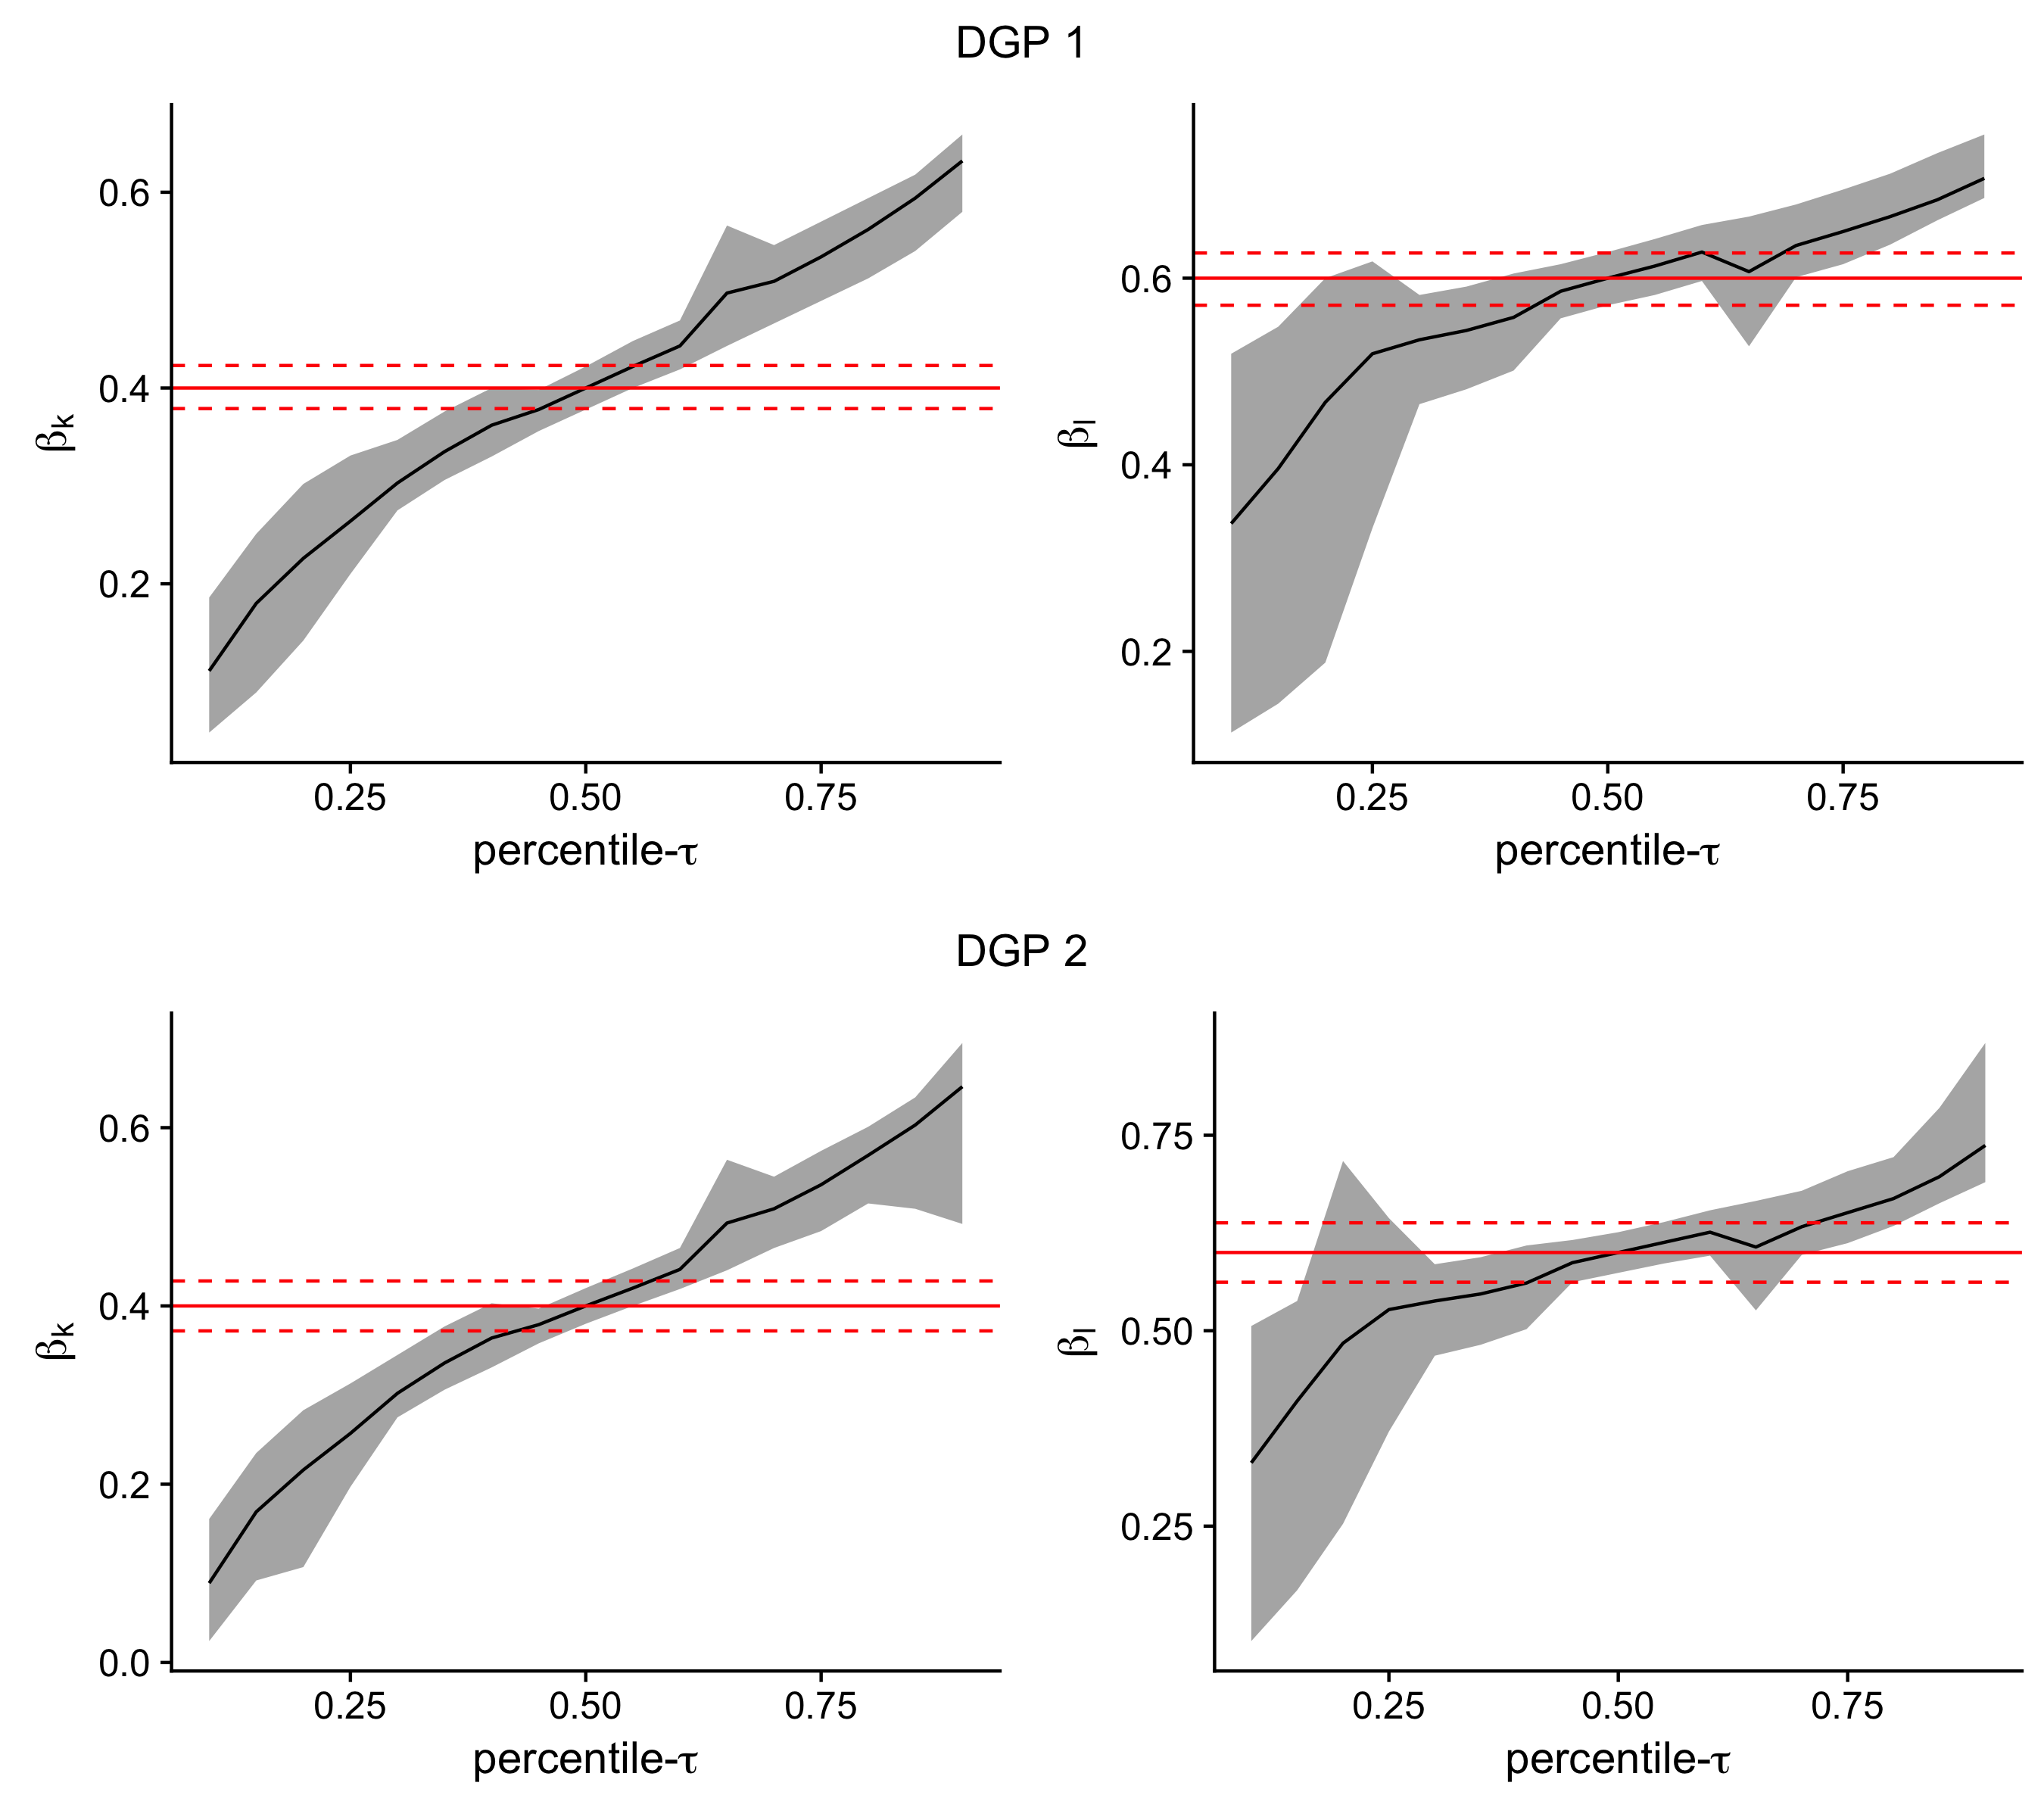
\includegraphics[width=11cm, height=9cm]{ACF_Coefficient_Plot.png}
\label{ACF_coefficient_plot}
\end{figure}

\begin{figure}[H]
\centering
\caption{Simulated precision of QACF estimators of $\beta_{k}(\tau)$ and $\beta_{l}(\tau)$s. Dotted line is ACF estimator.}
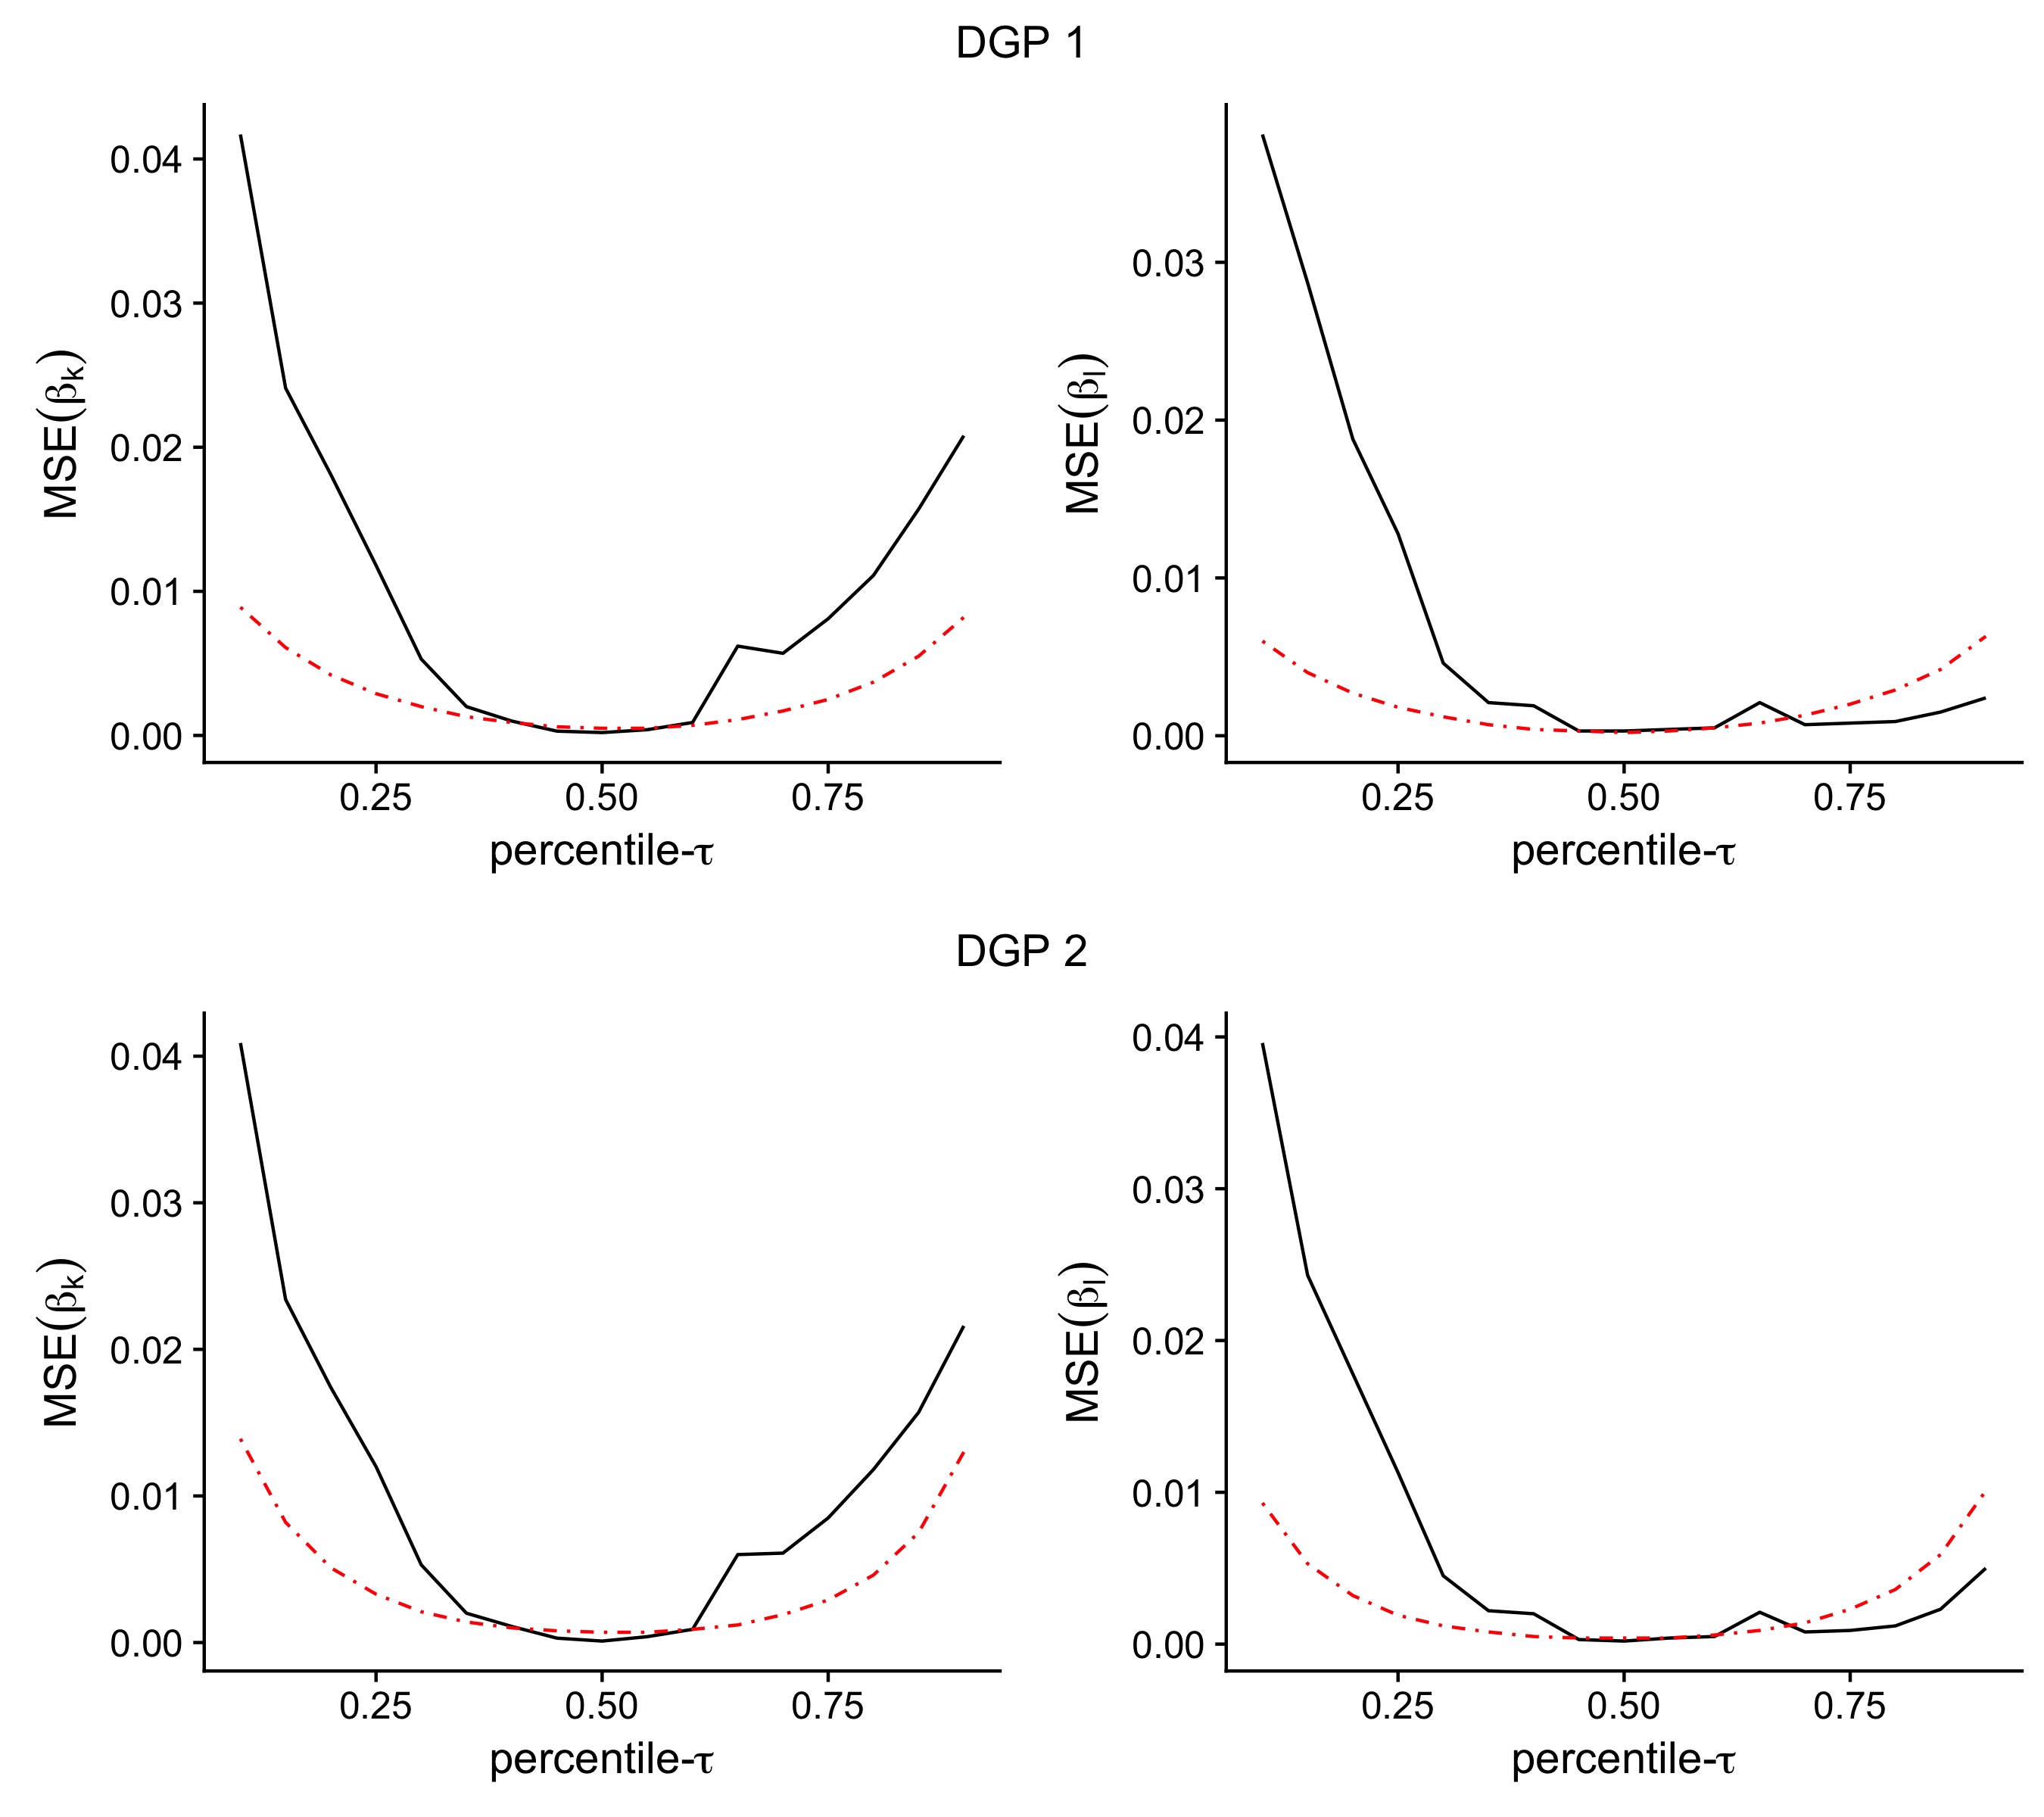
\includegraphics[width=11cm, height=9cm]{ACF_MSE_Plot.png}
\label{MSE_plot}
\end{figure}

\begin{figure}[H]
\centering
\caption{QLP estimated coefficients of  $\beta_{k}(\tau)$ and $\beta_{l}(\tau)$. Dotted line is LP estimator}
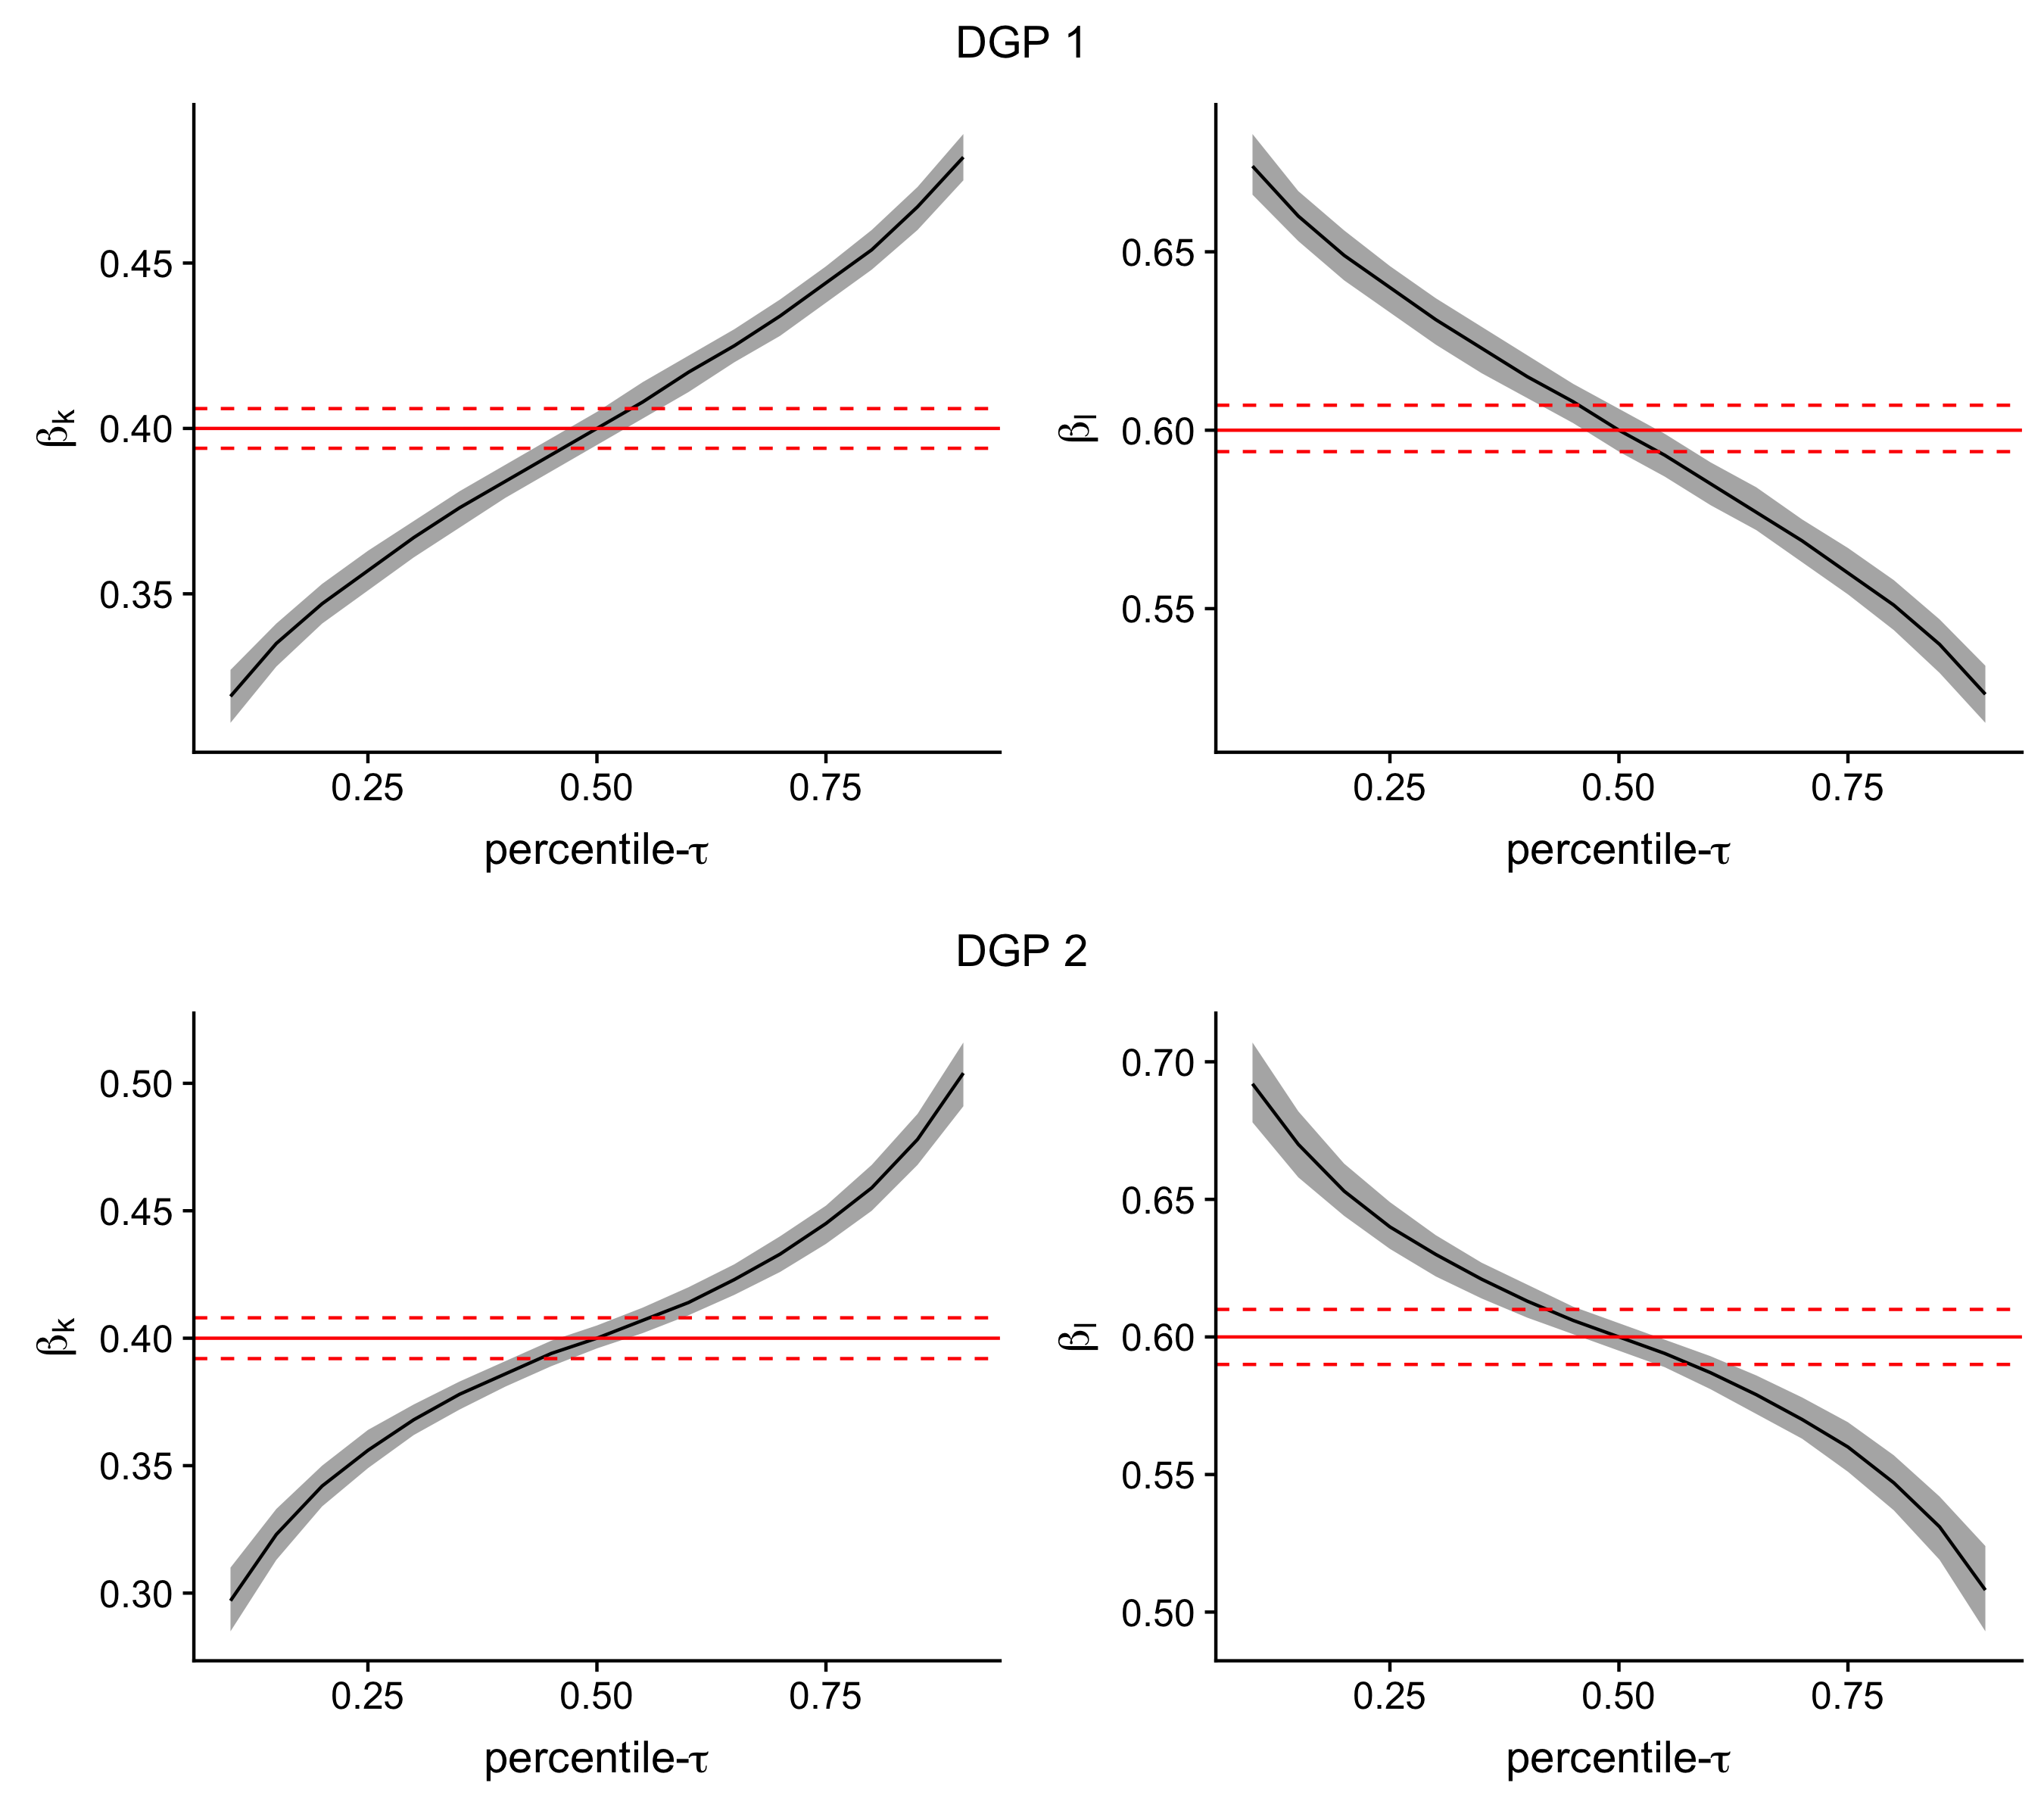
\includegraphics[width=11cm, height=9cm]{LP_Coefficient_Plot.png}
\label{LP_coefficient_plot}
\end{figure}


\begin{figure}[H]
\centering
\caption{Simulated precision of  QLP estimators of $\beta_{k}(\tau)$ and $\beta_{l}(\tau)$s. Dotted line is LP estimator.}
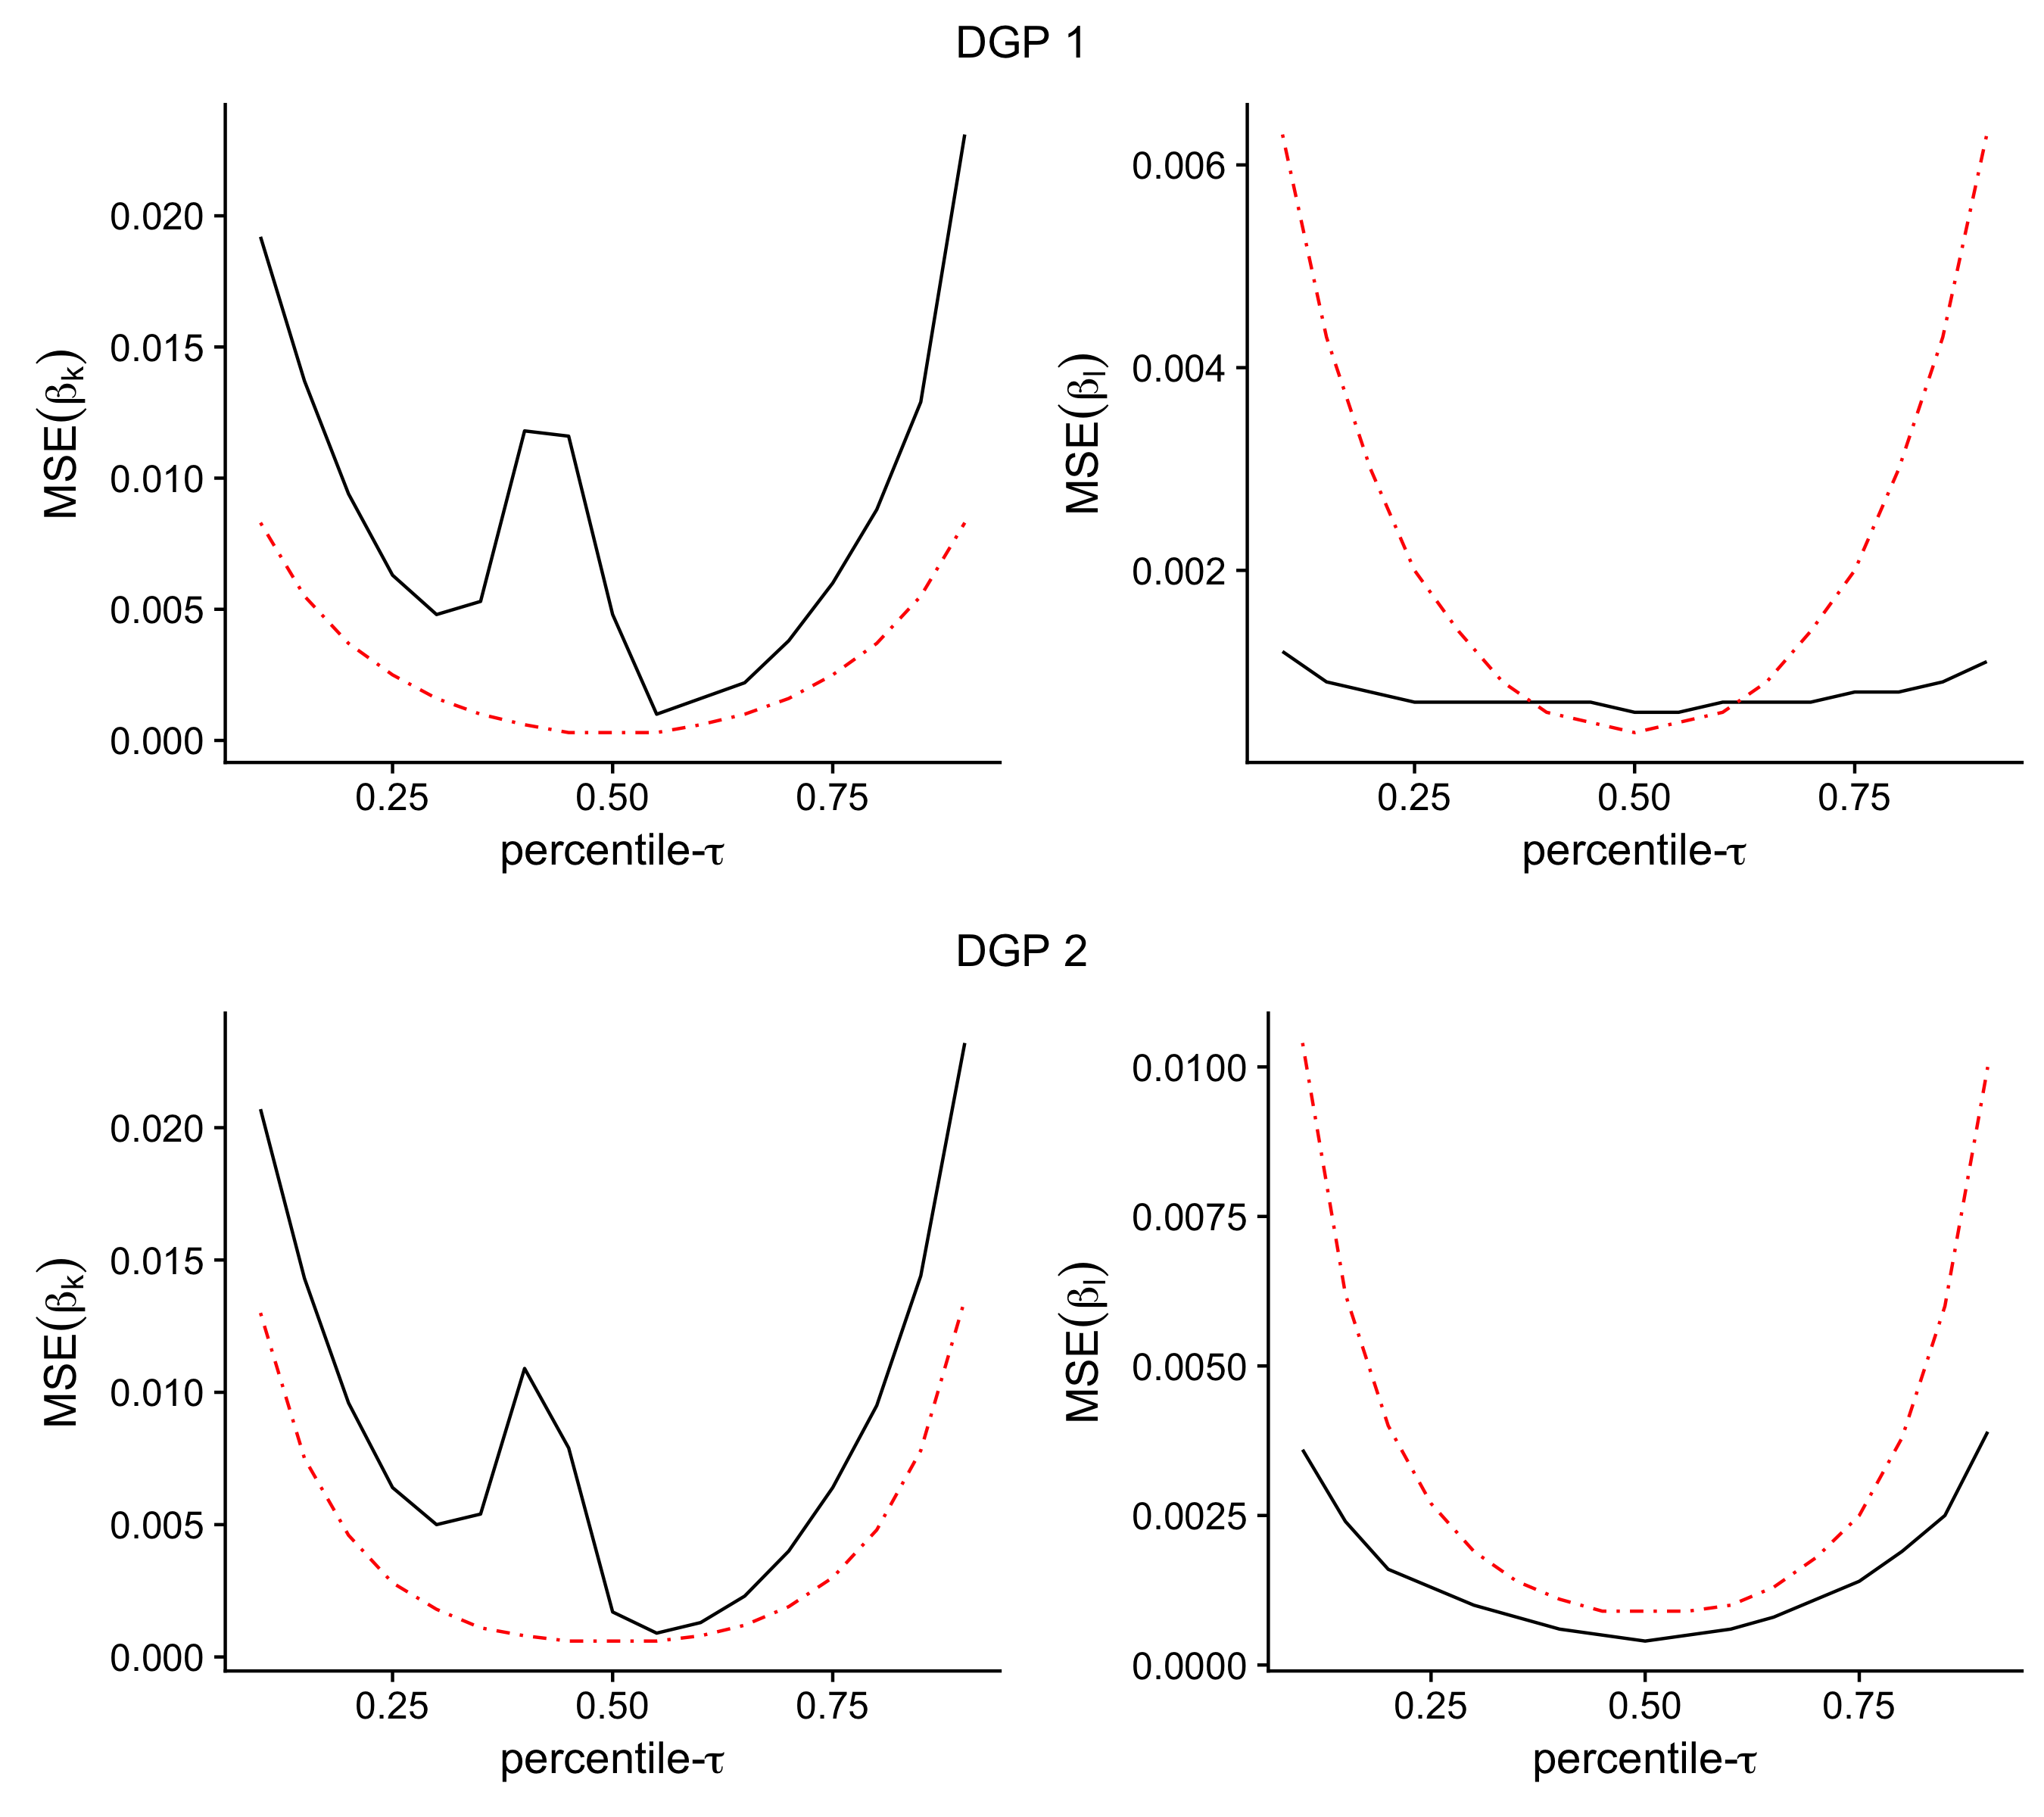
\includegraphics[width=11cm, height=9cm]{LP_MSE_Plot.png}
\label{MSE_plot}
\end{figure}


The next figure summarizes distributional information from our Monte Carlo experiment. These simulation results show that our estimator has good finite-sample performance and does reasonably well at capturing firm heterogeneity across quantiles.

\begin{figure}[H]
\centering
\caption{ACF Box Plots for estimated coefficients from 1000 replications of Monte Carlo}
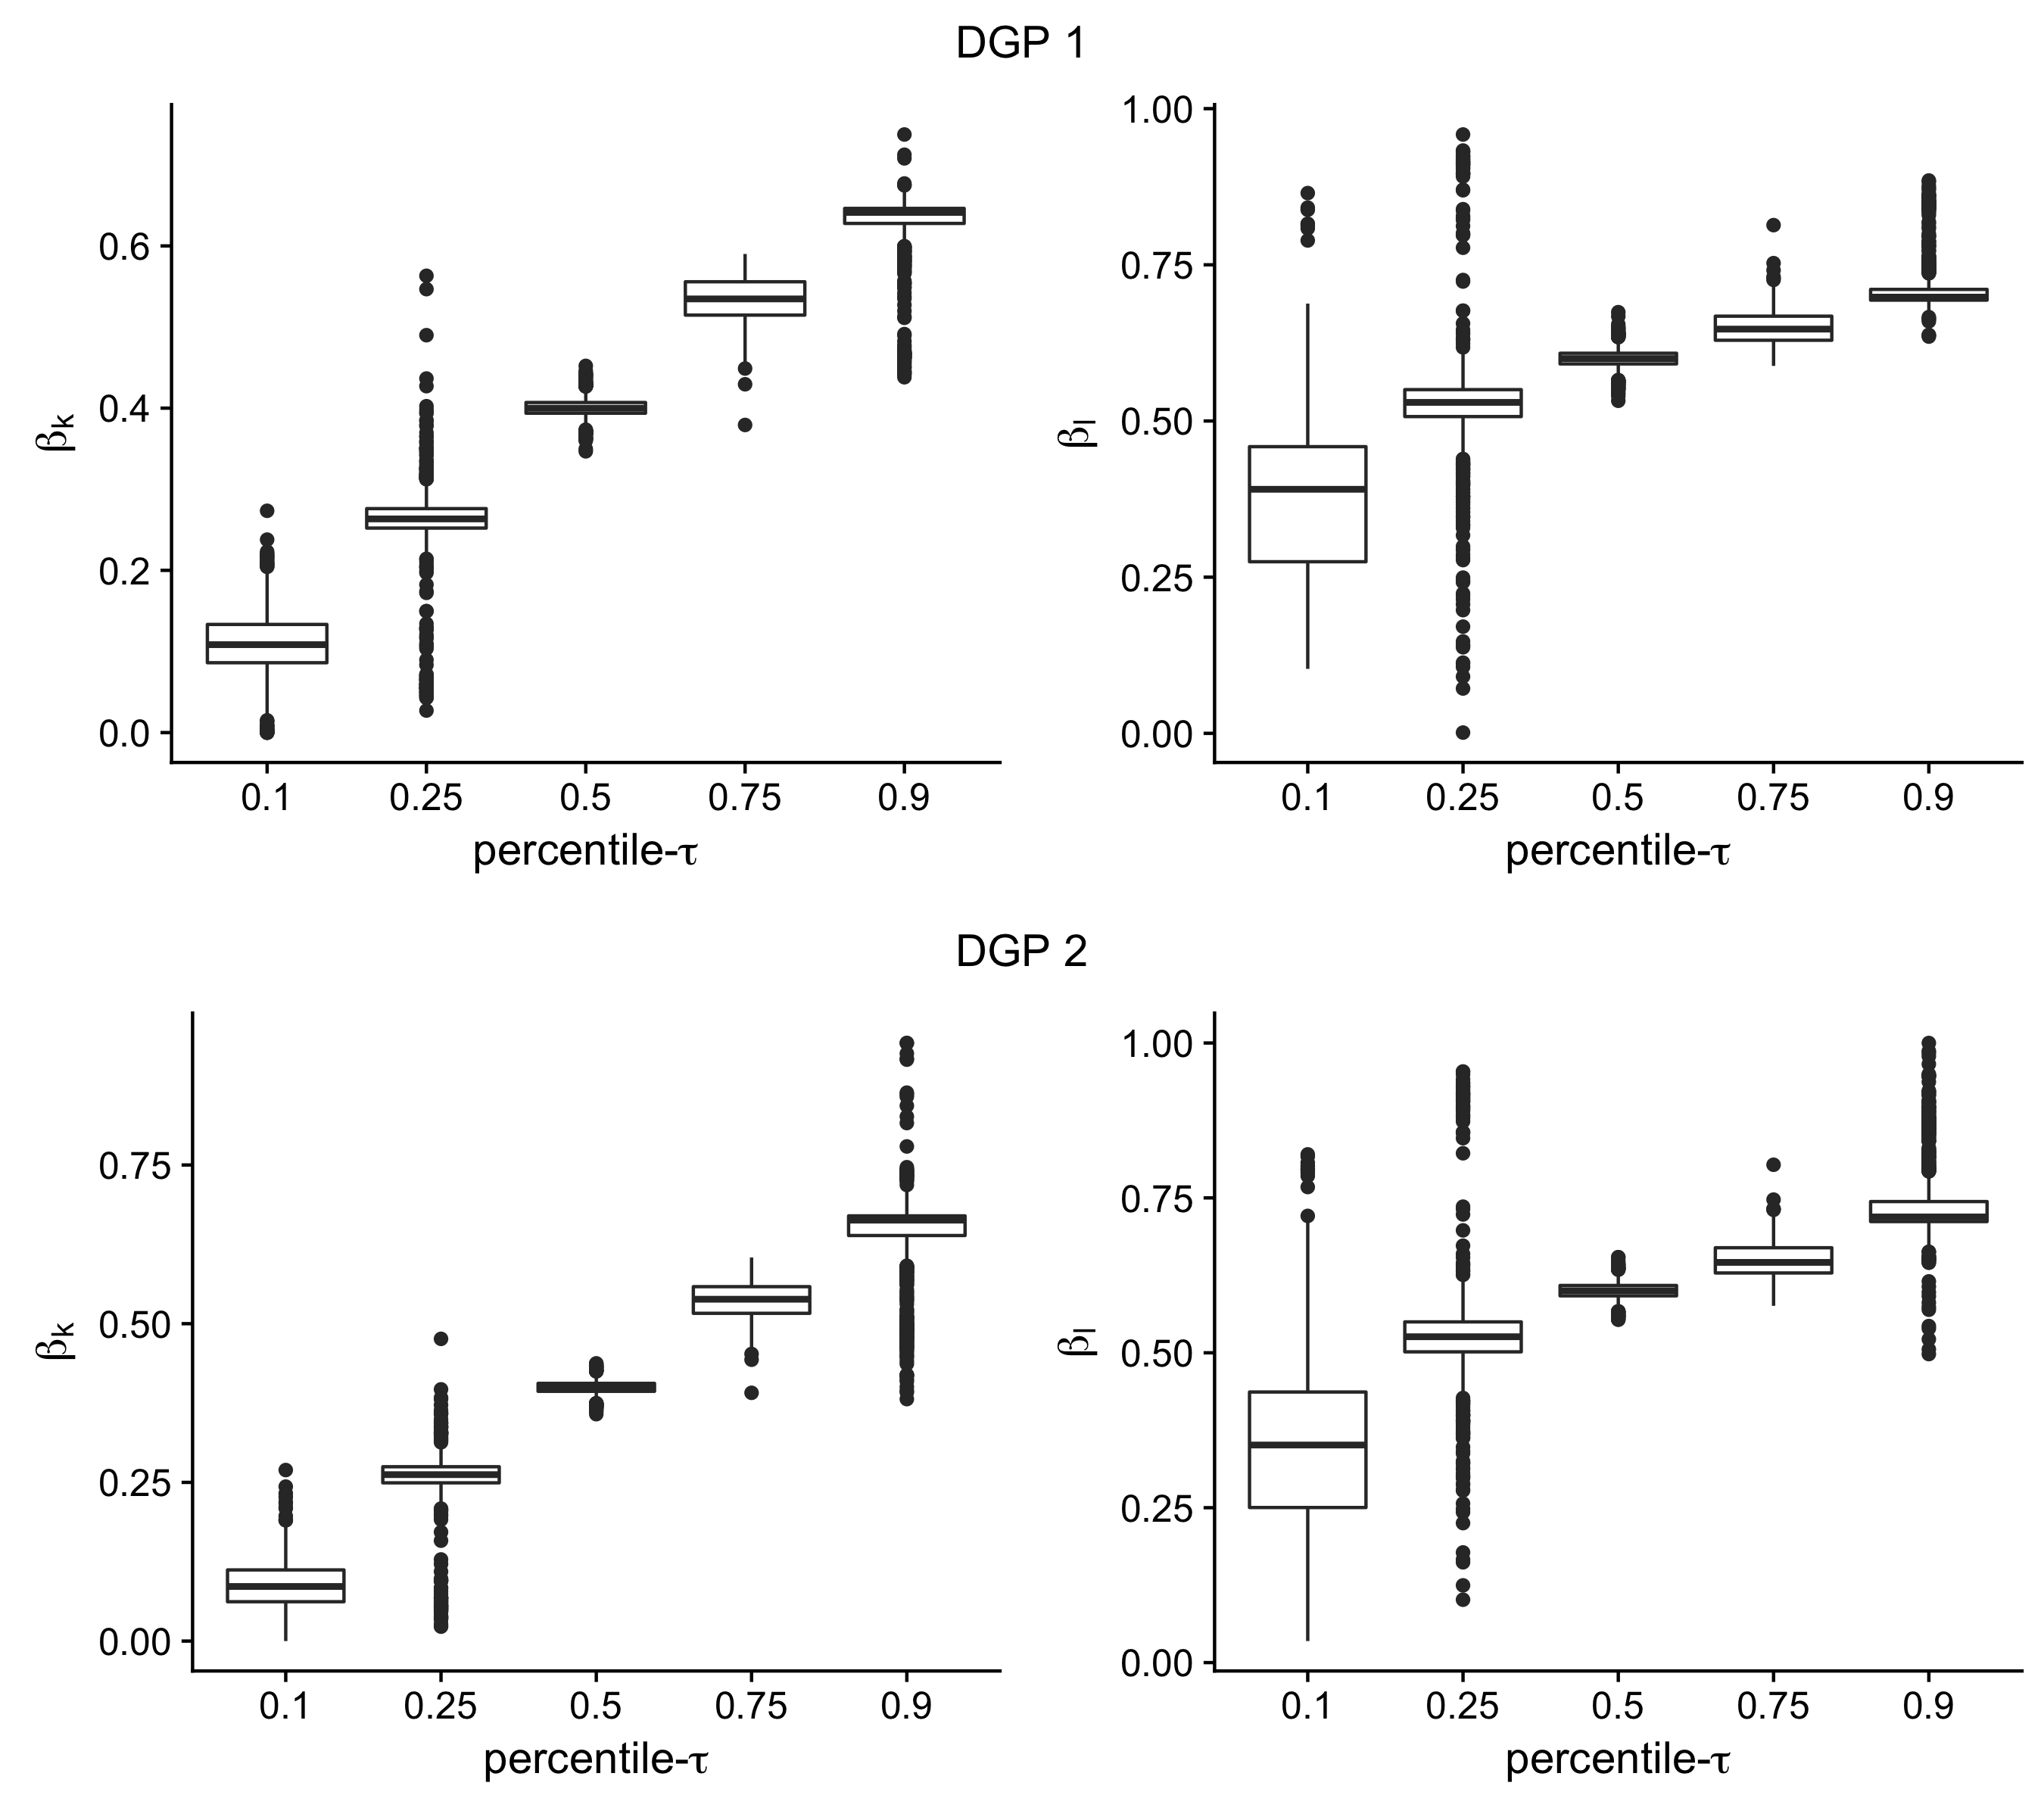
\includegraphics[width=12cm]{QACF_Box_Plot.png}
\label{ACF_Box Plot}
\end{figure}

\begin{figure}[H]
\centering
\caption{LP Box Plots for estimated coefficients from 1000 replications of Monte Carlo}
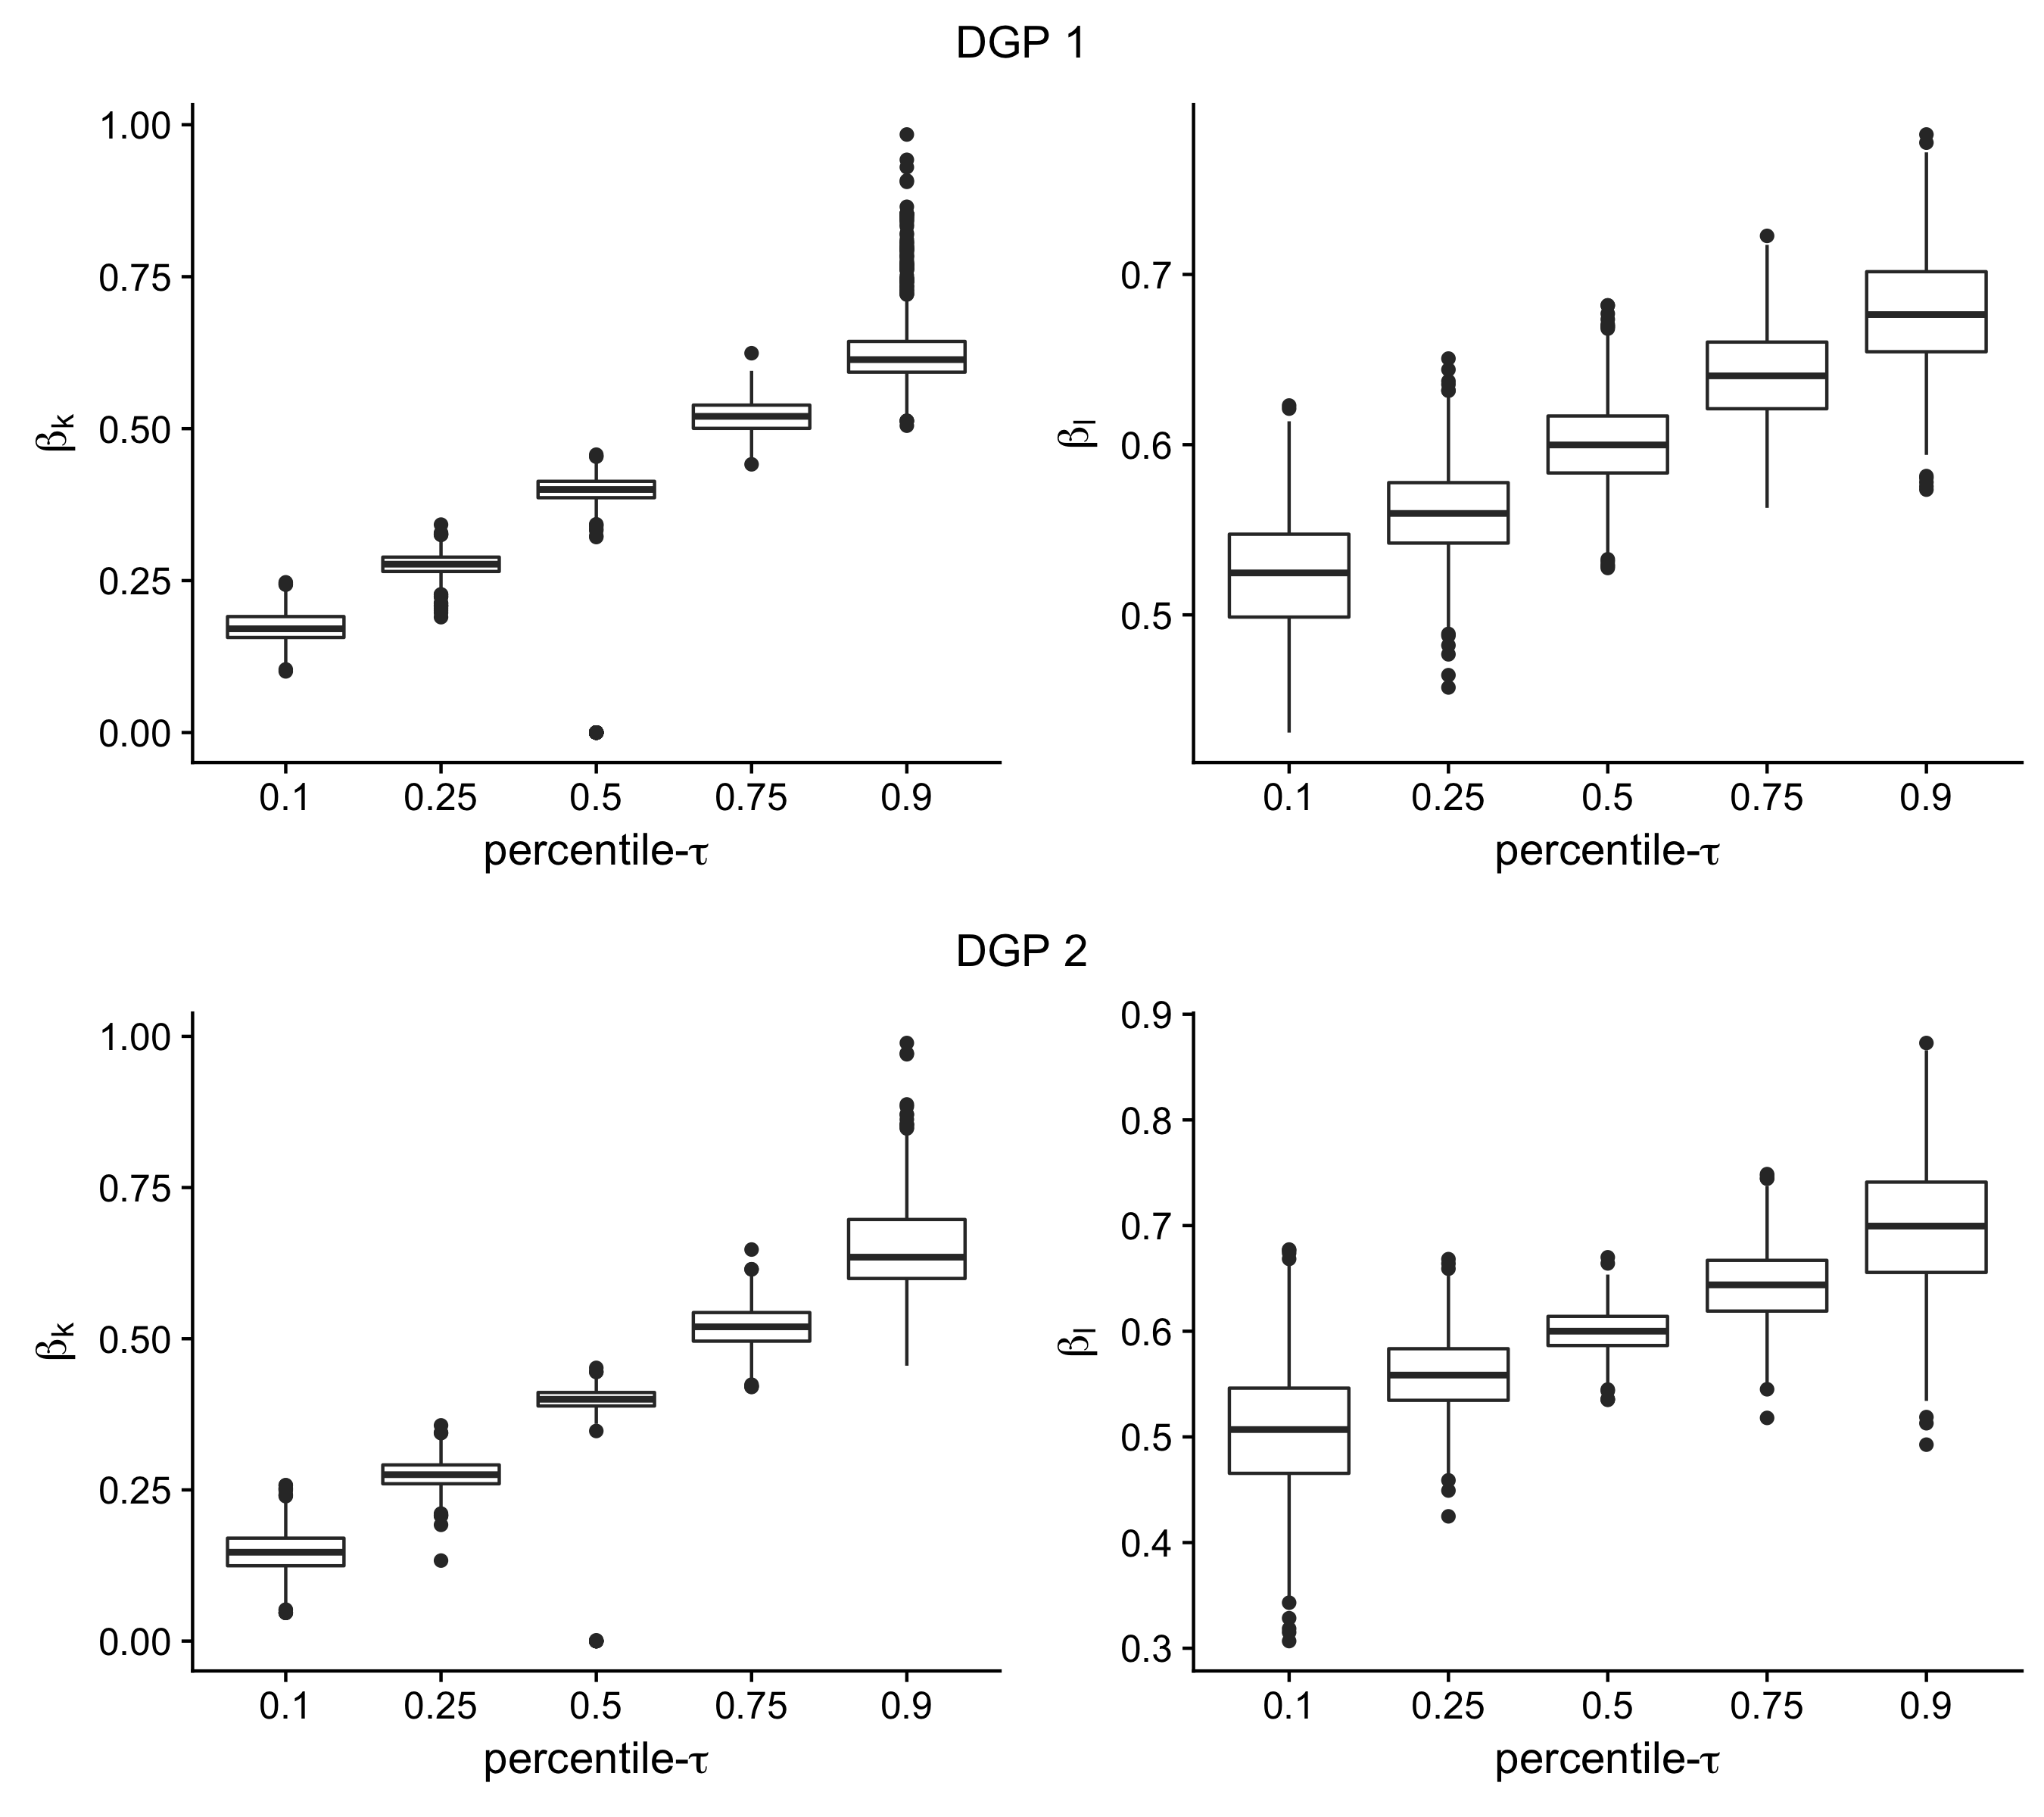
\includegraphics[width=12cm]{QLP_Box_Plot.png}
\label{LP_Box Plot}
\end{figure}

\section{Application}

\begin{table}[ht]
\centering
\begin{tabular}{cccccccccc}
  \hline\hline & & \multicolumn{2}{c}{Capital}  & \multicolumn{2}{c}{Skilled Labor} & \multicolumn{2}{c}{Unskilled Labor} & \multicolumn{2}{c}{Returns to Scale} \\ \cmidrule(lr){3-4} \cmidrule(lr){5-6} \cmidrule(lr){7-8} \cmidrule(lr){9-10}Industry (ISIC code) & $\tau$ & Coef. & s.e. & Coef. & s.e. & Coef. & s.e. & Coef. & s.e \\ 
  \hline
311 & 0.10 & 0.278 & 0.0570 & 0.313 & 0.0402 & 0.516 & 0.0443 & 1.107 & 0.0793 \\ 
   & 0.25 & 0.126 & 0.0375 & 0.274 & 0.0249 & 0.464 & 0.0298 & 0.865 & 0.0490 \\ 
   & 0.50 & 0.235 & 0.0444 & 0.246 & 0.0187 & 0.429 & 0.0241 & 0.909 & 0.0522 \\ 
   & 0.75 & 0.235 & 0.0561 & 0.209 & 0.0206 & 0.417 & 0.0263 & 0.861 & 0.0652 \\ 
  381 & 0.10 & 0.166 & 0.1123 & 0.465 & 0.0846 & 0.596 & 0.0772 & 1.228 & 0.1188 \\ 
   & 0.25 & 0.371 & 0.0981 & 0.393 & 0.0534 & 0.524 & 0.0675 & 1.288 & 0.1063 \\ 
   & 0.50 & 0.244 & 0.0783 & 0.399 & 0.0401 & 0.417 & 0.0469 & 1.061 & 0.0838 \\ 
   & 0.75 & 0.218 & 0.0622 & 0.367 & 0.0347 & 0.396 & 0.0305 & 0.981 & 0.0707 \\ 
  321 & 0.10 & 0.262 & 0.1278 & 0.545 & 0.0585 & 0.476 & 0.0692 & 1.283 & 0.1351 \\ 
   & 0.25 & 0.160 & 0.1144 & 0.511 & 0.0521 & 0.385 & 0.0558 & 1.056 & 0.1126 \\ 
   & 0.50 & 0.171 & 0.0665 & 0.492 & 0.0495 & 0.386 & 0.0545 & 1.049 & 0.0778 \\ 
   & 0.75 & 0.227 & 0.0613 & 0.442 & 0.0524 & 0.392 & 0.0627 & 1.061 & 0.0744 \\ 
  331 & 0.10 & 0.208 & 0.1020 & 0.435 & 0.0522 & 0.583 & 0.0728 & 1.225 & 0.1271 \\ 
   & 0.25 & 0.144 & 0.0662 & 0.378 & 0.0610 & 0.481 & 0.0676 & 1.003 & 0.0942 \\ 
   & 0.50 & 0.176 & 0.0580 & 0.351 & 0.0396 & 0.431 & 0.0498 & 0.959 & 0.0742 \\ 
   & 0.75 & 0.127 & 0.0600 & 0.378 & 0.0365 & 0.314 & 0.0410 & 0.819 & 0.0683 \\ 
   \hline
\end{tabular}
\end{table}

\begin{figure}[H]
\centering
\caption{Estimated values of production function coefficients and their 90\% confidence interval}
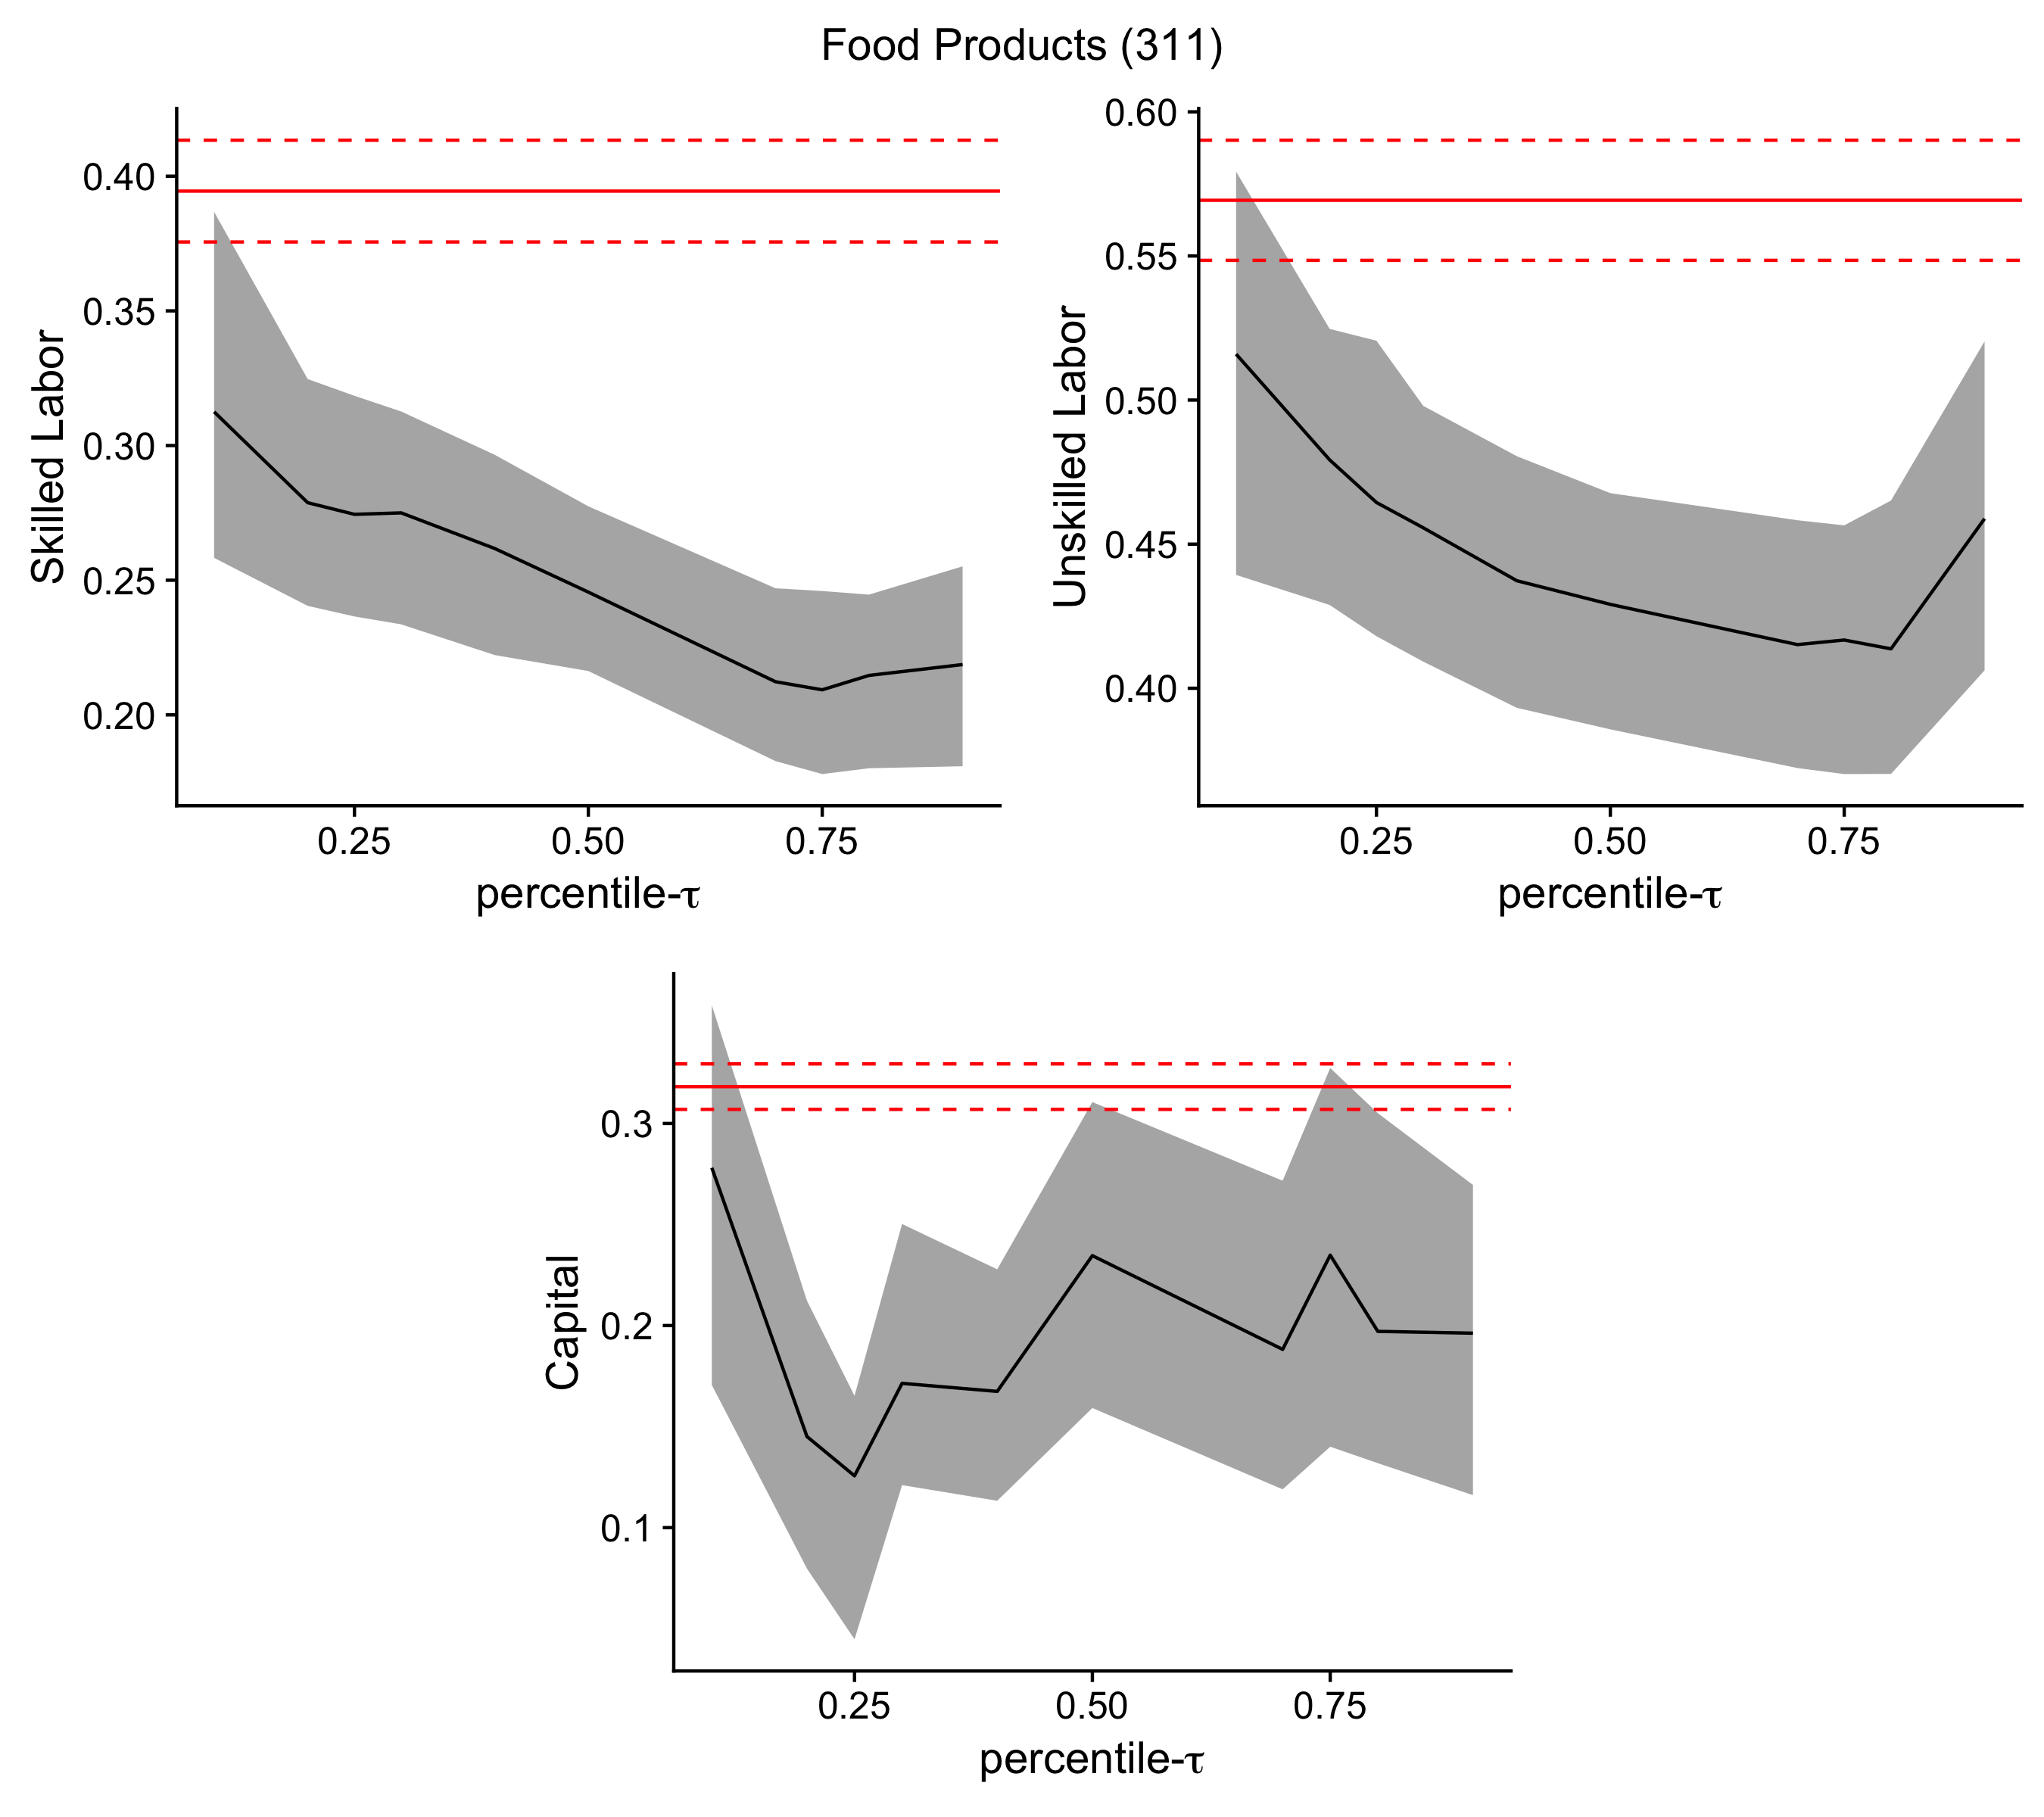
\includegraphics[width=12cm]{Coefficient_Plot_1.png}
\end{figure}

\begin{figure}[H]
\centering
\caption{Estimated values of production function coefficients and their 90\% confidence interval}
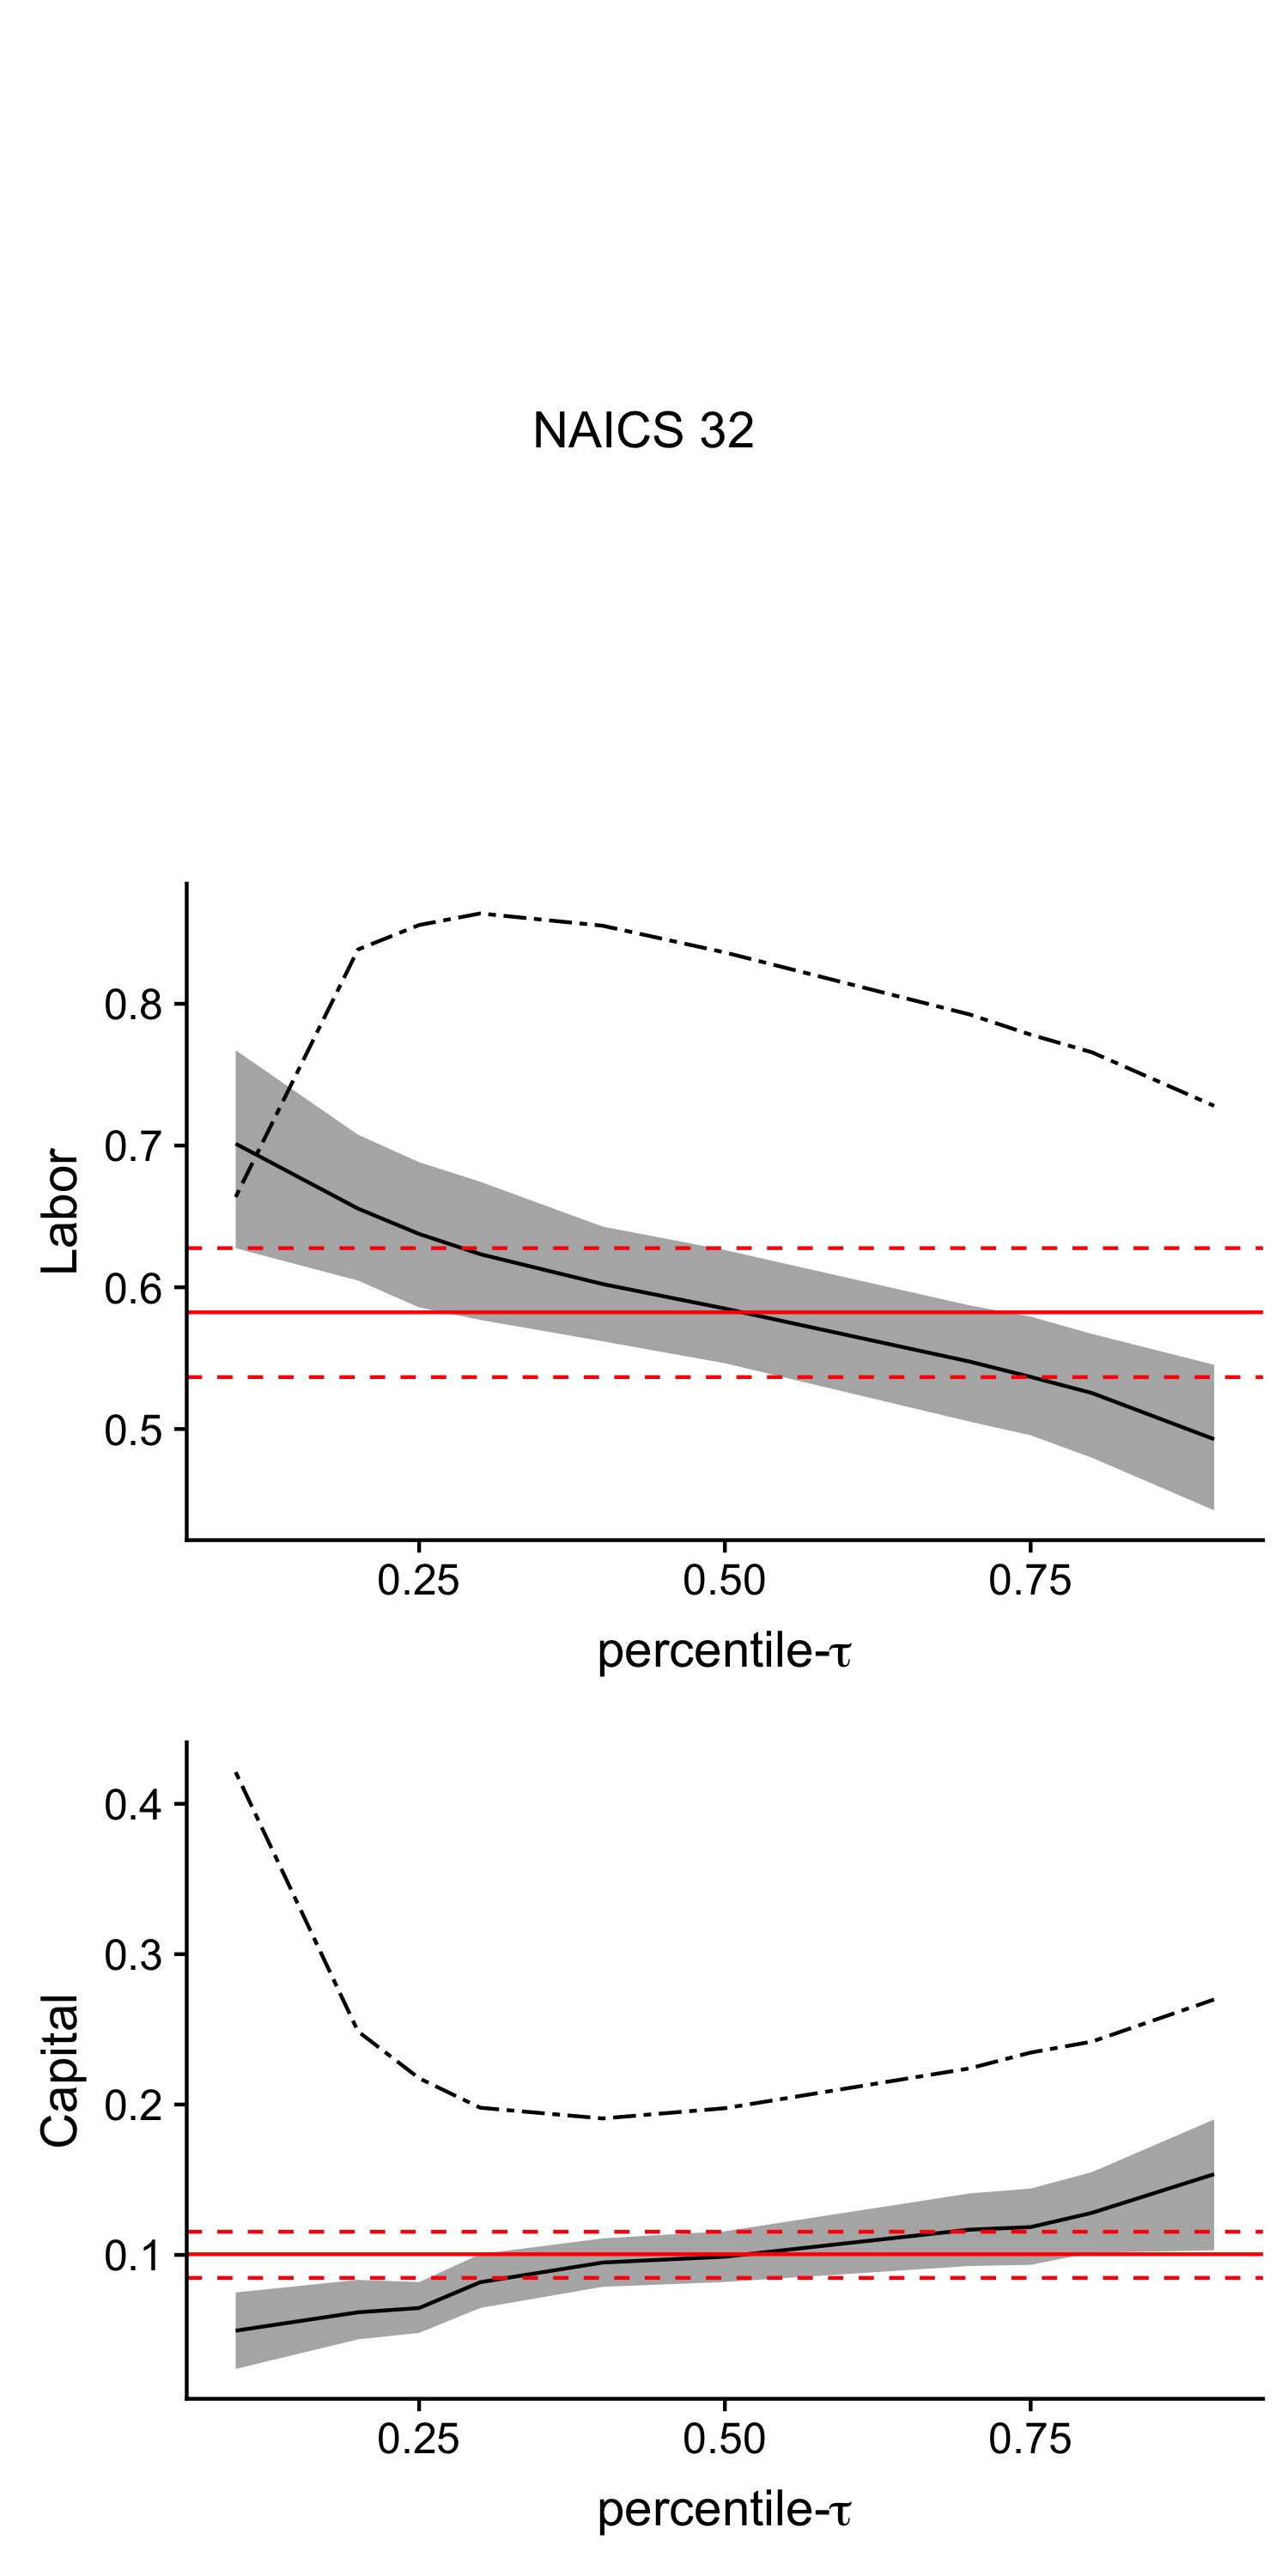
\includegraphics[width=12cm]{Coefficient_Plot_2.png}
\end{figure}

\begin{figure}[H]
\centering
\caption{Estimated values of production function coefficients and their 90\% confidence interval}
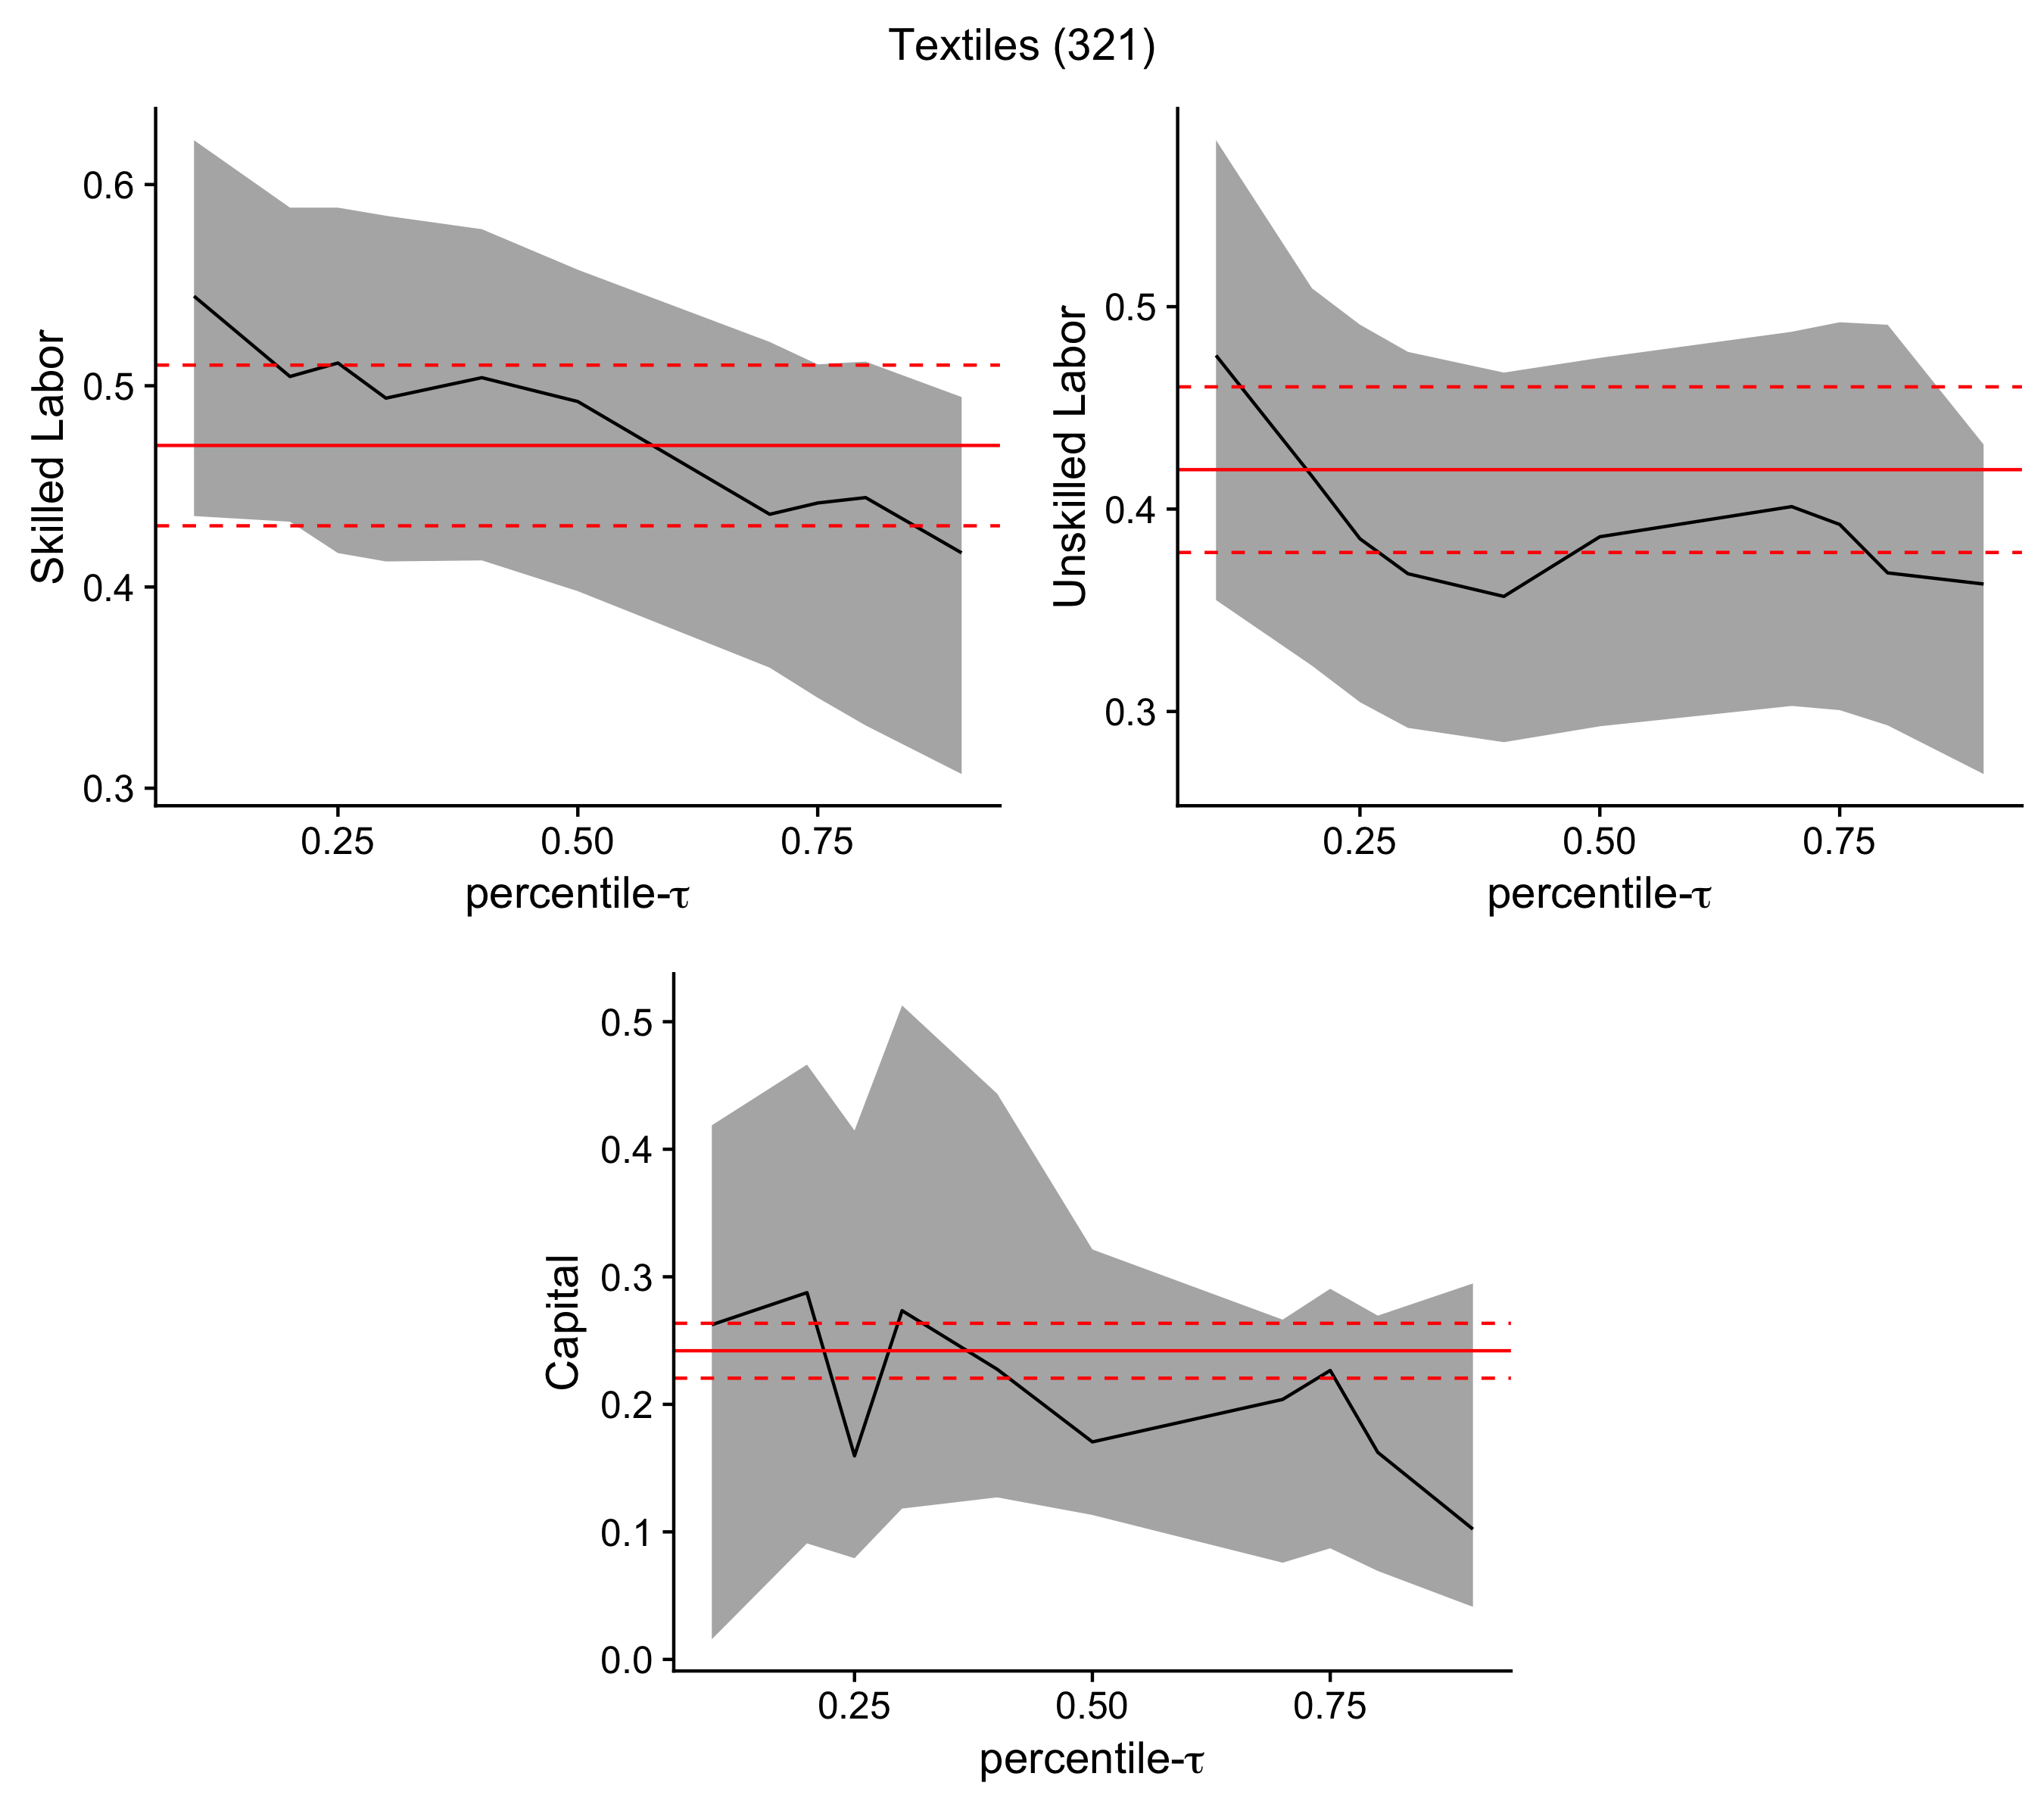
\includegraphics[width=12cm]{Coefficient_Plot_3.png}
\end{figure}

\begin{figure}[H]
\centering
\caption{Estimated values of production function coefficients and their 90\% confidence interval}
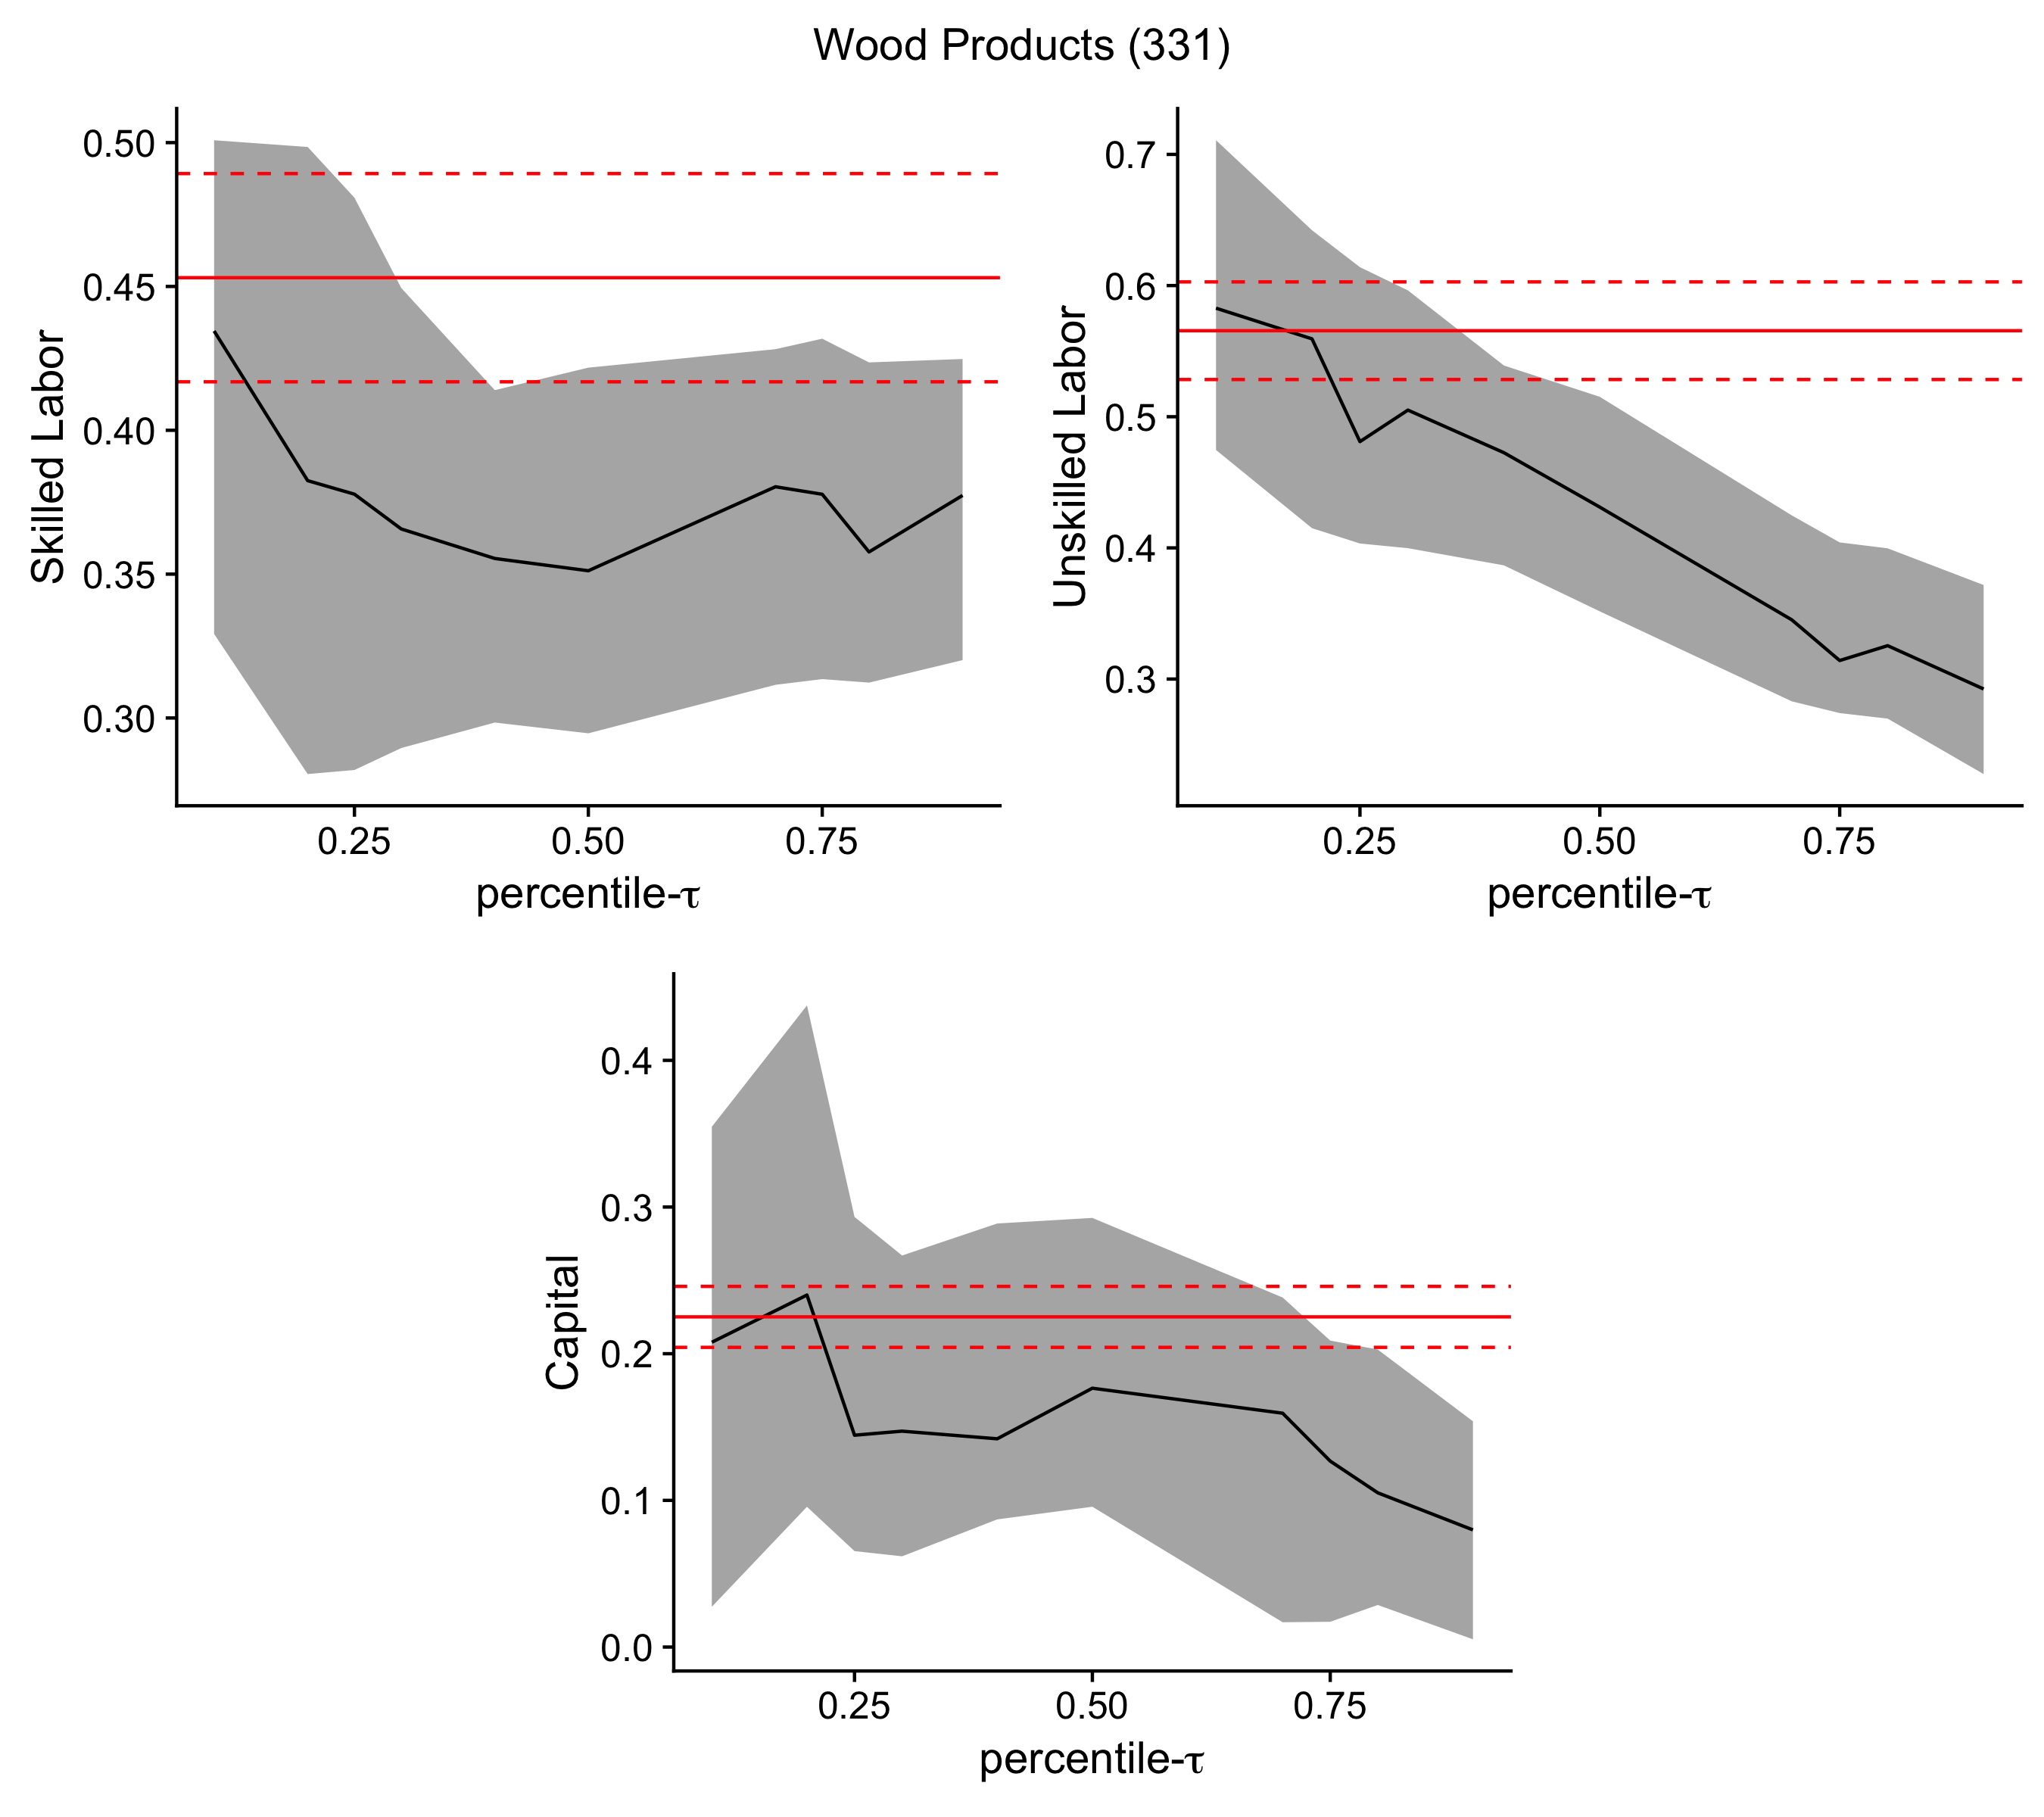
\includegraphics[width=12cm]{Coefficient_Plot_4.png}
\end{figure}

\section{Conclusions}

We proposed a method that extends the intermediate input proxy variable approach to estimating quantiles of the conditional quantiles of firm production. The method is computationally attractive as it resembles the two-stage estimator introduced in the control function literature with conditional quantile restrictions at each stage. As a result, practitioners are able to easily apply the proposed estimator to production function models where the data reveal significant heterogeneous output elasticities along the conditional distribution of firm's output. We showed that this estimator works well in finite samples by replicating the experiment of ACF (2015) and showing that it captures heterogeneity in firm-size under different data generating processes.  

Econometric issues with this estimator are currently being explored. A method to consistently estimate the long-run variance of the sample moment conditions to achieve the semi-parametric efficiency bound under general conditions is desired and extending the asymptotic results of \cite*{qgmm} might not be straightforward. We also seek to estimate and interpret the resulting estimates of total factor productivity. Once these are addressed, an application using data such as the Chilean firm-level data may reveal heterogeneity in production technology along the distribution of firm output. 
We leave them as future research agenda.


\pagebreak
\newpage



%\section*{Appendix}
%\appendix
%\begin{Large}
%\noindent \textbf{A. Proof of the Theorems}
%\end{Large}

%\counterwithin{theorem}{section}
%\section{Proofs}





\bibliographystyle{ecca.bst}
\bibliography{references}




\end{document}